\documentclass[a4paper,12pt]{article}
\usepackage{datetime}
\usepackage{amsmath, amsthm, amssymb}
\usepackage[dvipsnames]{xcolor}
\usepackage{tikz} % 添加绘图
\usepackage{tabularx}
\usepackage{enumitem}
\usepackage{fancyref}

\usepackage[top=1in,bottom=1in,left=1in,right=1in]{geometry} % 用于设置页面布局
\usepackage{xeCJK} % 用于使用本地字体
\usepackage[super, square, sort&compress]{natbib} % 处理参考文献
\usepackage{titlesec, titletoc} % 设置章节标题及页眉页脚
%\usepackage{xCJKnumb} % 中英文数字转换
\usepackage{amssymb}
\usepackage{amsmath} % 在公式中用\text{文本}输入中文
\usepackage{diagbox}
\usepackage{multirow} % 表格中使用多行
\usepackage{booktabs} % 表格中使用\toprule等命令
\usepackage{rotating} % 使用sidewaystable环境旋转表格
\usepackage{tabularx}
\usepackage{graphicx} % 处理图片
\usepackage{footnote} % 增强的脚注功能,可添加表格脚注
\usepackage{threeparttable} % 添加真正的表格脚注,示例见README
\usepackage{hyperref} % 添加pdf书签

\usepackage{tikz}
\usetikzlibrary{shapes,arrows,shadows}

% 字体设置
\setmainfont{Times New Roman}
\setsansfont[Scale=MatchLowercase,Mapping=tex-text]{PT Sans}
\setmonofont[Scale=MatchLowercase]{PT Mono}
\setCJKmainfont[ItalicFont={Kaiti SC}, BoldFont={Heiti SC}]{Songti SC}
\setCJKsansfont{Heiti SC}
\setCJKmonofont{Songti SC}
% \setCJKmainfont[BoldFont={FZXiaoBiaoSong-B05S}]{Songti SC}
% \setCJKfamilyfont{kai}[BoldFont=Heiti SC]{Kaiti SC}
% \setCJKfamilyfont{song}[BoldFont=Heiti SC]{Songti SC}
% \setCJKfamilyfont{hei}[BoldFont=Heiti SC]{Heiti SC}
% \setCJKfamilyfont{fsong}[BoldFont=Heiti SC]{Songti SC}
% \newcommand{\kai}[1]{{\CJKfamily{kai}#1}}
% \newcommand{\hei}[1]{{\CJKfamily{hei}#1}}
% \setromanfont[Mapping=tex-text]{TeXGyrePagella}
% \setsansfont[Scale=MatchLowercase,Mapping=tex-text]{TeXGyrePagella}
% \setmonofont[Scale=MatchLowercase]{Courier New}
%%设置常用中文字号,方便调用
\newcommand{\erhao}{\fontsize{22pt}{\baselineskip}\selectfont}
\newcommand{\xiaoerhao}{\fontsize{18pt}{\baselineskip}\selectfont}
\newcommand{\sanhao}{\fontsize{16pt}{\baselineskip}\selectfont}
\newcommand{\xiaosanhao}{\fontsize{15pt}{\baselineskip}\selectfont}
\newcommand{\sihao}{\fontsize{14pt}{\baselineskip}\selectfont}
\newcommand{\xiaosihao}{\fontsize{12pt}{\baselineskip}\selectfont}
\newcommand{\wuhao}{\fontsize{10.5pt}{\baselineskip}\selectfont}
\newcommand{\xiaowuhao}{\fontsize{9pt}{\baselineskip}\selectfont}
\newcommand{\liuhao}{\fontsize{7.5pt}{\baselineskip}\selectfont}

% 章节标题显示方式及页眉页脚设置
% \item xCJKnumb是自己额外安装的包
% \item titleformat命令定义标题的形式
% \item titlespacing定义标题距左、上、下的距离
\titleformat{\section}{\raggedright\large\bfseries}{\thesection}{1em}{}
\titleformat{\subsection}{\raggedright\normalsize\bfseries}{\thesubsection}{1em}{}
\titlespacing{\section}{0pt}{*0}{*2}
\titlespacing{\subsection}{0pt}{*0}{*1}
% 由于默认的2em缩进不够,所以我手动调整了,但是在windows下似乎2.2就差不多了,或者是article中没有这个问题
\setlength{\parindent}{2.2em}

% 设置表格标题前后间距
\setlength{\abovecaptionskip}{0pt}
\setlength{\belowcaptionskip}{0pt}


\renewcommand{\refname}{\bfseries{参~考~文~献}} %将Reference改为参考文献(用于 article)
% \renewcommand{\bibname}{参~考~文~献} %将bibiography改为参考文献(用于 book)
\renewcommand{\baselinestretch}{1.38} %设置行间距
\renewcommand{\figurename}{\small\ttfamily 图}
\renewcommand{\tablename}{\small\ttfamily 表}


\setlength{\parindent}{0em}

\newcommand{\specialcell}[2][c]{%
  \begin{tabular}[#1]{@{}c@{}}#2\end{tabular}}

\newtheorem{lemma}{引理}
\newtheorem{proposition}{命题}
\newtheorem{grammar}{文法}
\newtheorem{program}{程序}
\newtheorem{convention}{约定}
\renewcommand*{\proofname}{证明}

\usetikzlibrary{shapes.geometric}
\tikzset{
    turtle/.style={
        draw,
        shape border rotate=270,
        regular polygon,
        regular polygon sides=3,
        fill=gray,
        node distance=2cm,
        minimum height=4em
    }
}

\newdateformat{monthyeardate}{\THEYEAR 年 \THEMONTH 月}

\title{在庞加莱圆盘上看加法与乘法}
\author{苑明理}
\date{\monthyeardate\today}

\begin{document}

\maketitle{}

\renewcommand\contentsname{目录}
\setcounter{tocdepth}{2}
\tableofcontents

\newpage

\section{预备知识}

\subsection{数的一种表示}

我们采用逆波兰表达式的记法,用两个操作 b 和 m ,以及初始操作数 0 和 1 ,来表示出不同的数字,其中:

\begin{convention}
正向操作
\begin{itemize}
\item b 表示加一的操作
\item m 表示乘二的操作
\end{itemize}
\end{convention}

我们作示例如下表

\begin{table}[tbhp]
\centering
\begin{tabularx}{\textwidth}
{|>{\setlength\hsize{0.95\hsize}\setlength\linewidth{\hsize}}X
 |>{\setlength\hsize{0.95\hsize}\setlength\linewidth{\hsize}}X
 |>{\setlength\hsize{0.95\hsize}\setlength\linewidth{\hsize}}X
 |>{\setlength\hsize{0.95\hsize}\setlength\linewidth{\hsize}}X
 |>{\setlength\hsize{0.95\hsize}\setlength\linewidth{\hsize}}X
 |>{\setlength\hsize{0.95\hsize}\setlength\linewidth{\hsize}}X
 |>{\setlength\hsize{0.95\hsize}\setlength\linewidth{\hsize}}X|}
\hline
数字 & 1 &  2 &  3 &  4 &  5 & 6 \\
\hline
不同表示 &
\begin{itemize}[leftmargin=*]\item 0b\end{itemize} &
\begin{itemize}[leftmargin=*]\item 0bb\item 1m\end{itemize} &
\begin{itemize}[leftmargin=*]\item 0bbb\item 1mb\end{itemize} &
\begin{itemize}[leftmargin=*]\item 0bbbb\item 1mbb\item 0bbm\item 1mm\end{itemize} &
\begin{itemize}[leftmargin=*]\item 0bbbbb\item 1mbbb\item 0bbmb\item 1mmb\end{itemize} &
\begin{itemize}[leftmargin=*]\item 0bbbbbb\item 1mbbbb\item 0bbmbb\item 1mmbb\item 1mbm\end{itemize} \\
\hline
最简表示 & 0b & 1m & 1mb & 1mm & 1mmb & 1mbm \\
\hline
\end{tabularx}
\caption{六个自然数的表示}
\end{table}

生成自然数的合法的表达式可以由下述文法给出:

\begin{grammar}
\label{g1}
合法的表达式
\begin{itemize}
\item $E := (0 | 1)(b | m)*$
\end{itemize}
\end{grammar}

下面,我们引入操作 b 的逆操作 d ,操作 m 的逆操作 w

\begin{convention}
逆向操作
\begin{itemize}
\item d 表示减一的操作
\item w 表示除二的操作
\end{itemize}
\end{convention}

生成有理数的合法的表达式可以由下述文法给出:

\begin{grammar}
\label{g2}
合法的表达式
\begin{itemize}
\item $E := (0 | 1)(b | d | m | w)*$
\end{itemize}
\end{grammar}

初始操作数有 0 和 1 两个选择,大家可能会对此有一定的疑问。初始操作数 1 的引入主要是为了在求得最简表示时消除一些特定的例子。
在后面的章节,我们会取消初始操作数 1。


\subsection{操作序列的逆}

实际上,初始操作数可以放宽到任何一个有理数。我们假设操作数是 $\alpha$ ,操作序列是 $a_1 a_2 ... a_{n-1} a_n$ ,结果是 $\beta$ ,
在当前的记法下,我们写作 $\beta = \alpha a_1 a_2 ... a_{n-1} a_n$。

\begin{lemma}
\label{l1}
如果有 $\beta = \alpha a_1 a_2 ... a_{n-1} a_n$,则$\alpha = \beta a_n^{-1} a_{n-1}^{-1} ... a_2^{-1} a_1^{-1}$。
\end{lemma}

\begin{proof}
注意到 b、d、m、w 都是双射,我们知道操作序列 $\alpha a_1 a_2 ... a_{n-1} a_n$ 对应于函数的复合:

$$\beta = a_n( a_{n-1}( ... a_2( a_1(\alpha) ) ... ) )$$

考虑到函数复合的逆,我们有:

$$\alpha = a_1^{-1}( a_2^{-1}( ... a_{n-1}^{-1}( a_n^{-1}(\beta) ) ... ) )$$

在另外一个记法下,此即有,

$$\alpha = \beta a_n^{-1} a_{n-1}^{-1} ... a_2^{-1} a_1^{-1}$$

\qedhere

\end{proof}

\subsection{支持裂解的海龟绘图}

Logo 是一种程序设计语言,并以它的绘图执行环境而闻名。Logo 绘图执行环境的一个关键构造是绘图小海龟。
小海龟维持有一个指向,可以前进、后退若干步长,也可以左转、右转若干角度。

\begin{figure}[ht]
\centering
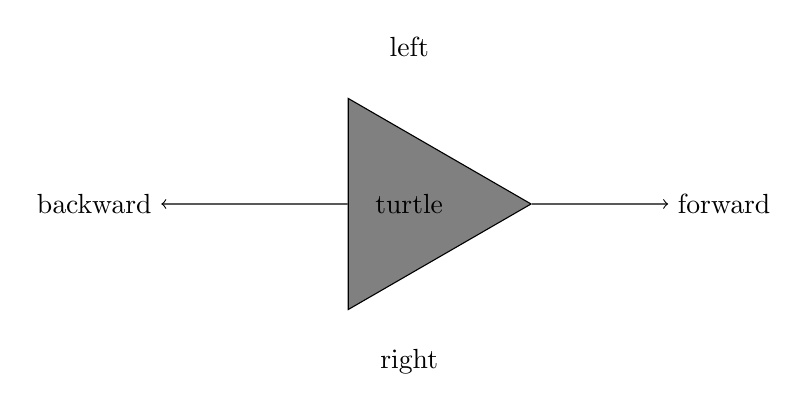
\begin{tikzpicture}

% nodes
\node (bk) at (4, 2) {backward};
\node[turtle] (tt) at (8, 2) {turtle};
\node (fd) at (12, 2) {forward};
\node (lt) at (8, 4) {left};
\node (rt) at (8, 0) {right};

% arrows
\draw[->] (tt) edge (bk);
\draw[->] (tt) edge (fd);

\end{tikzpicture}
\caption{绘图海龟的基本概念}
\end{figure}

许多分形构造或者镶嵌构造可以非常方便的通过一种支持裂解操作的 Logo 语言来实现。我们放宽原始 Logo 语言里的设定,
允许在画布上有多个海龟的存在,并且每个海龟单独维护自己的步长标准。于是,所谓的裂解是指一个操作,
它可以让一个海龟变成按照一定角度排布的多个海龟,同时新生成的海龟有新的步长设定。对于角度的排布,我们规定前进方向右侧转向是正的方向。

\begin{convention}
裂解采用如下的命令形式:
\begin{itemize}
\item 裂解[角度排布;步长设定]
\end{itemize}
\end{convention}

\subsection{四阶无限边形镶嵌}

双曲平面上有许多非常有趣的镶嵌结构,这里我们展示一种称为四阶无限边形镶嵌的构造。

\begin{figure}[ht]
\centering
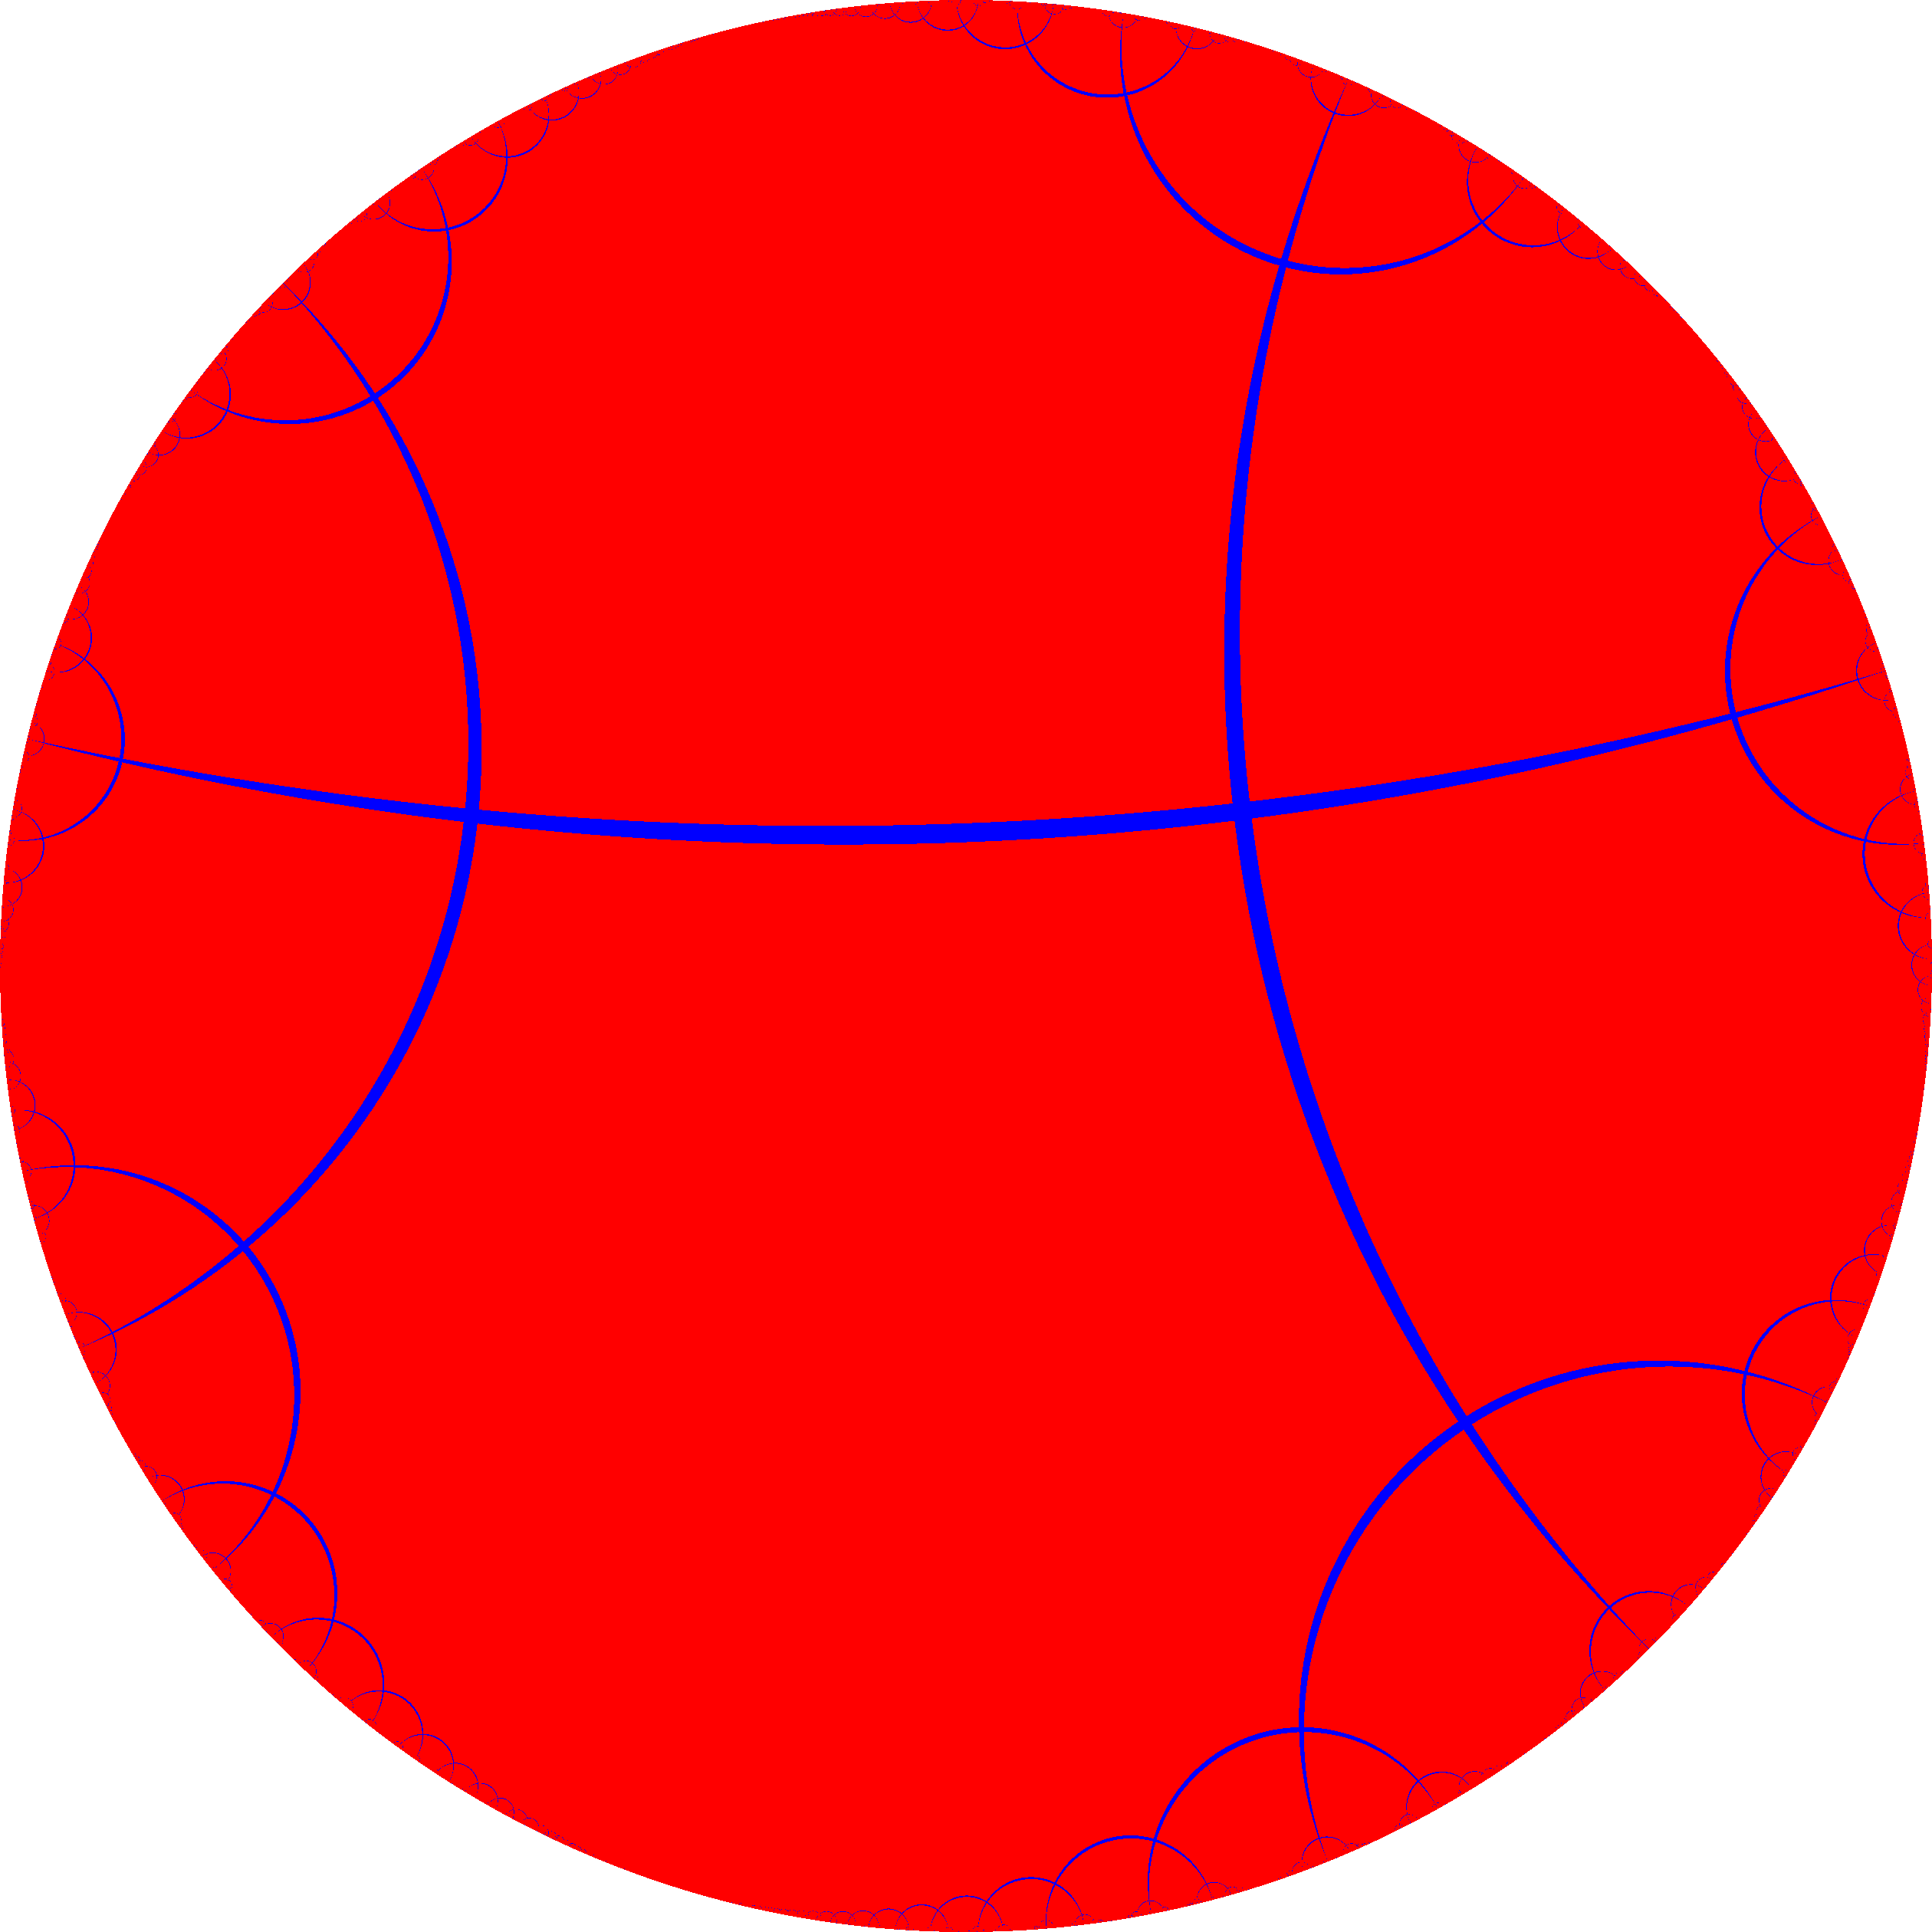
\includegraphics[width=3.5in]{images/H2_tiling_24i-1.png}
\caption{四阶无限边形镶嵌}
\end{figure}

这个镶嵌结构的构造程序如下

\begin{program}
四阶无限边形镶嵌的构造一
\begin{itemize}
\item 裂解[0, +90, +180, +270; 1]
\item 对所有的小海龟,反复无限次的执行下述命令
\begin{itemize}\item 前进一步 \item 裂解[-90, 0, +90; 1] \end{itemize}
\end{itemize}
\end{program}

如果注意到双曲平面是一个齐性空间,并且观察到在上述构造里,有些蓝色测地线之间彼此有交点,但这些交点彼此之间没有任何差别;
每一个交点都是两个测地线交汇出来的,都有四支分叉。利用对称性,我们容易理解:

\begin{proposition}
\label{A}
镶嵌结构上的两条测地线如果彼此之间相交,那么它们就是垂直的;否则这两条测地线就是平行的。
\end{proposition}

\begin{proposition}
\label{B}
对于任意一条镶嵌结构上的测地线,镶嵌结构上的其他测地线可以被归类到与之平行或垂直的两组之中。
\end{proposition}

\subsection{H-树}

H-树是如下图所示的分形构造。四阶无限边形镶嵌按照一定规则剪枝,拓扑上可以得到H-树。

\begin{figure}[ht]
\centering
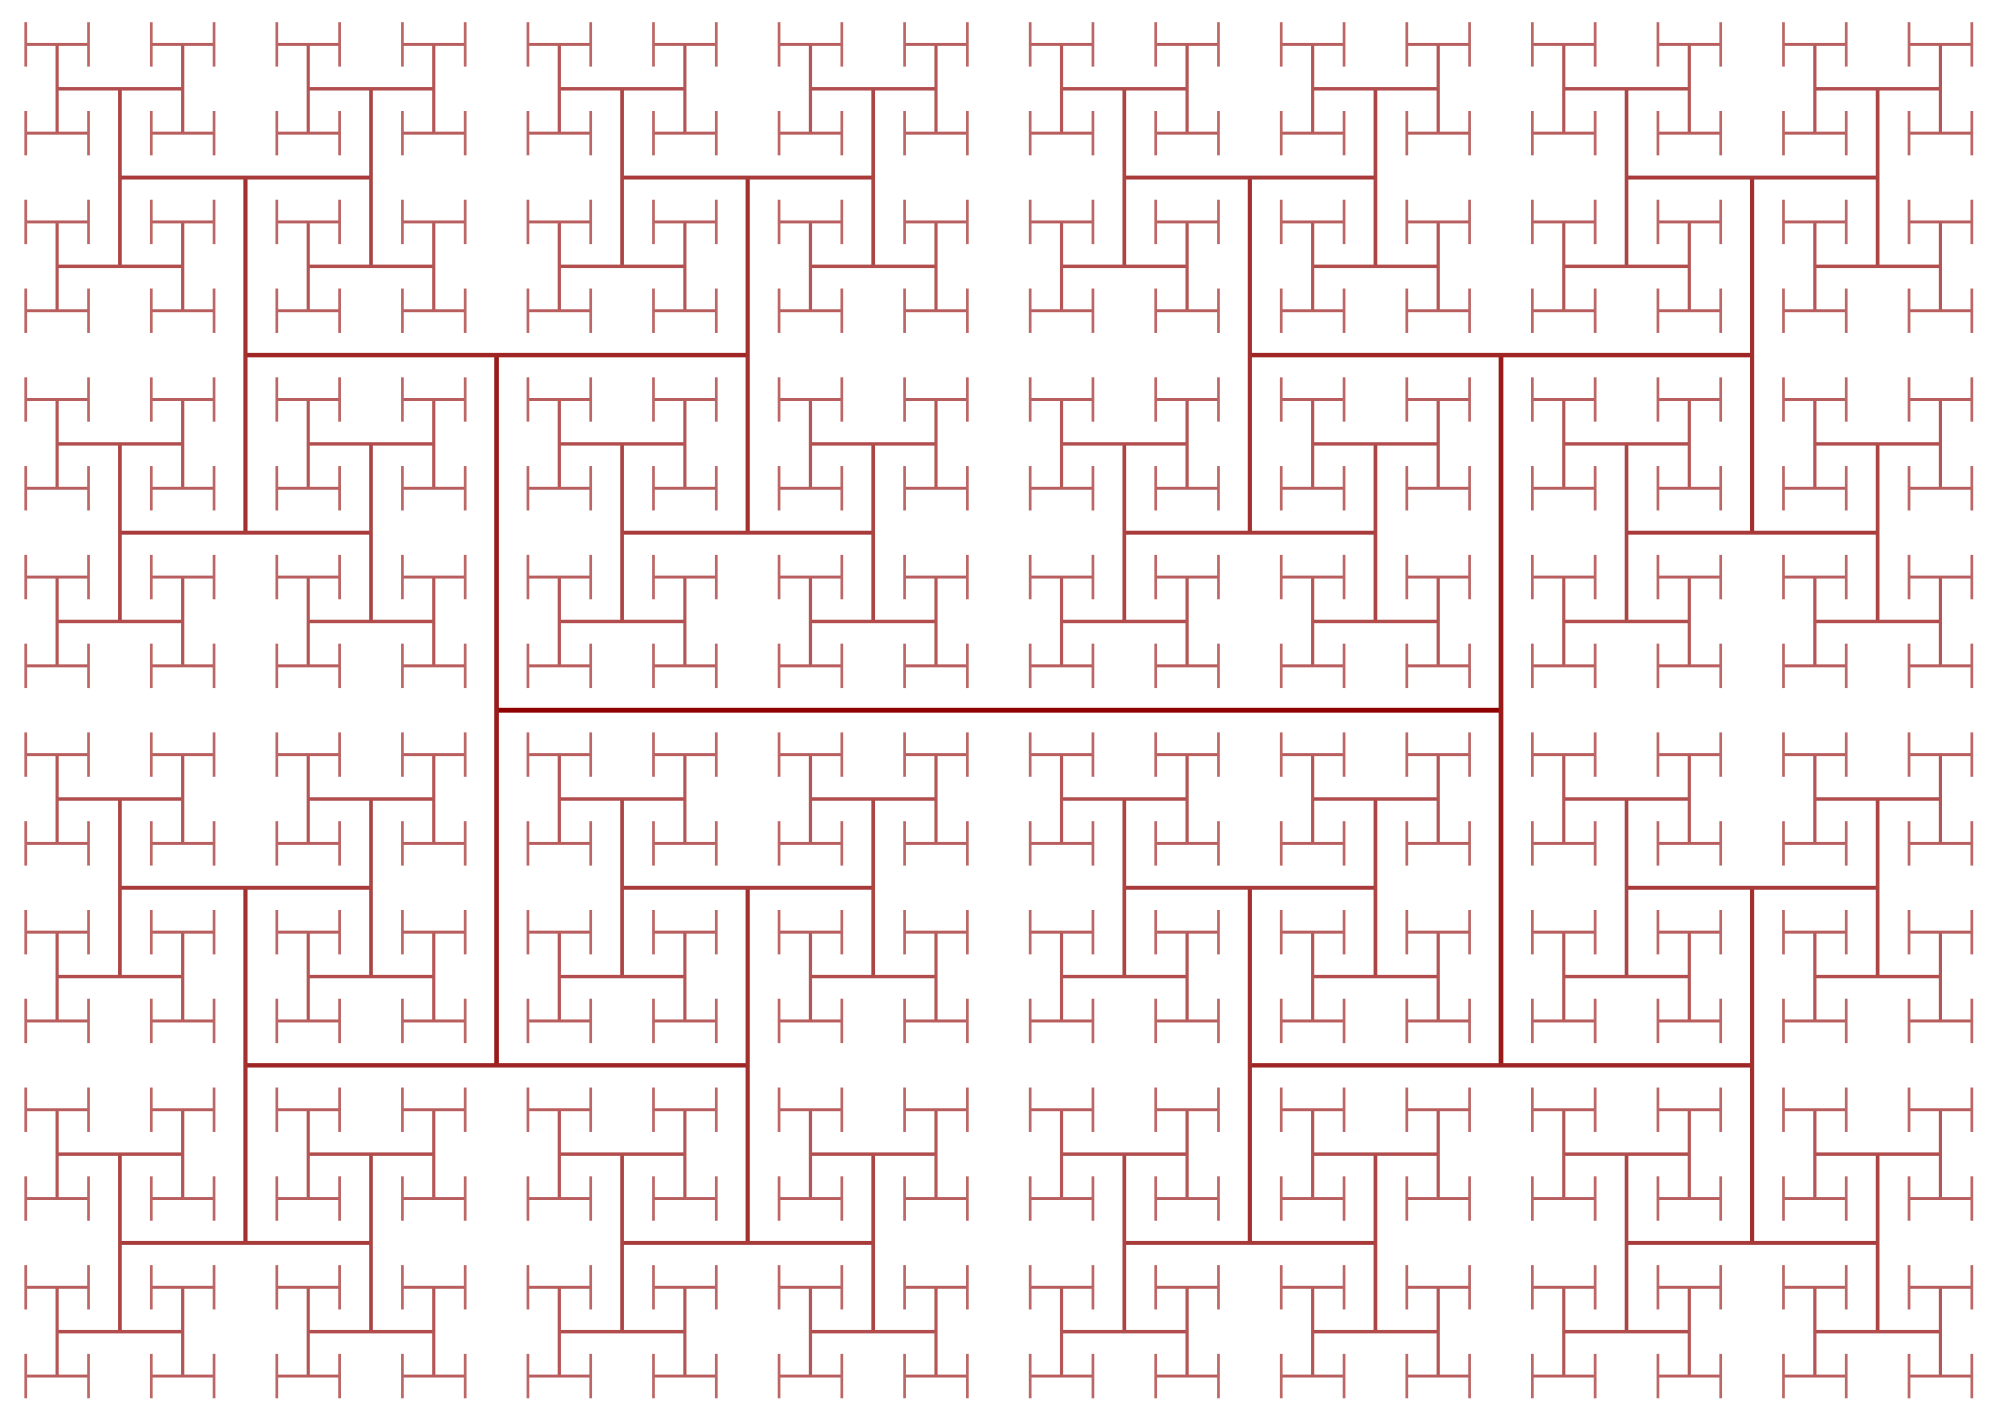
\includegraphics[width=3.5in]{images/2000px-H_tree.png}
\caption{H-树}
\end{figure}

H-树的具体构造程序如下

\begin{program}
H-树的构造
\begin{itemize}
\item 对所有的小海龟,反复无限次的执行下述命令
\begin{itemize}\item 前进一步 \item 裂解[-90, +90; $\sqrt{2} / 2$] \end{itemize}
\end{itemize}
\end{program}

\newpage

\subsection{镶嵌的其他方面}

\subsubsection{测地线 $\gamma$ 的六个无穷远点}

\begin{figure}[ht]
\centering
\begin{tikzpicture}
    \draw (0, 0) node[inner sep=0] {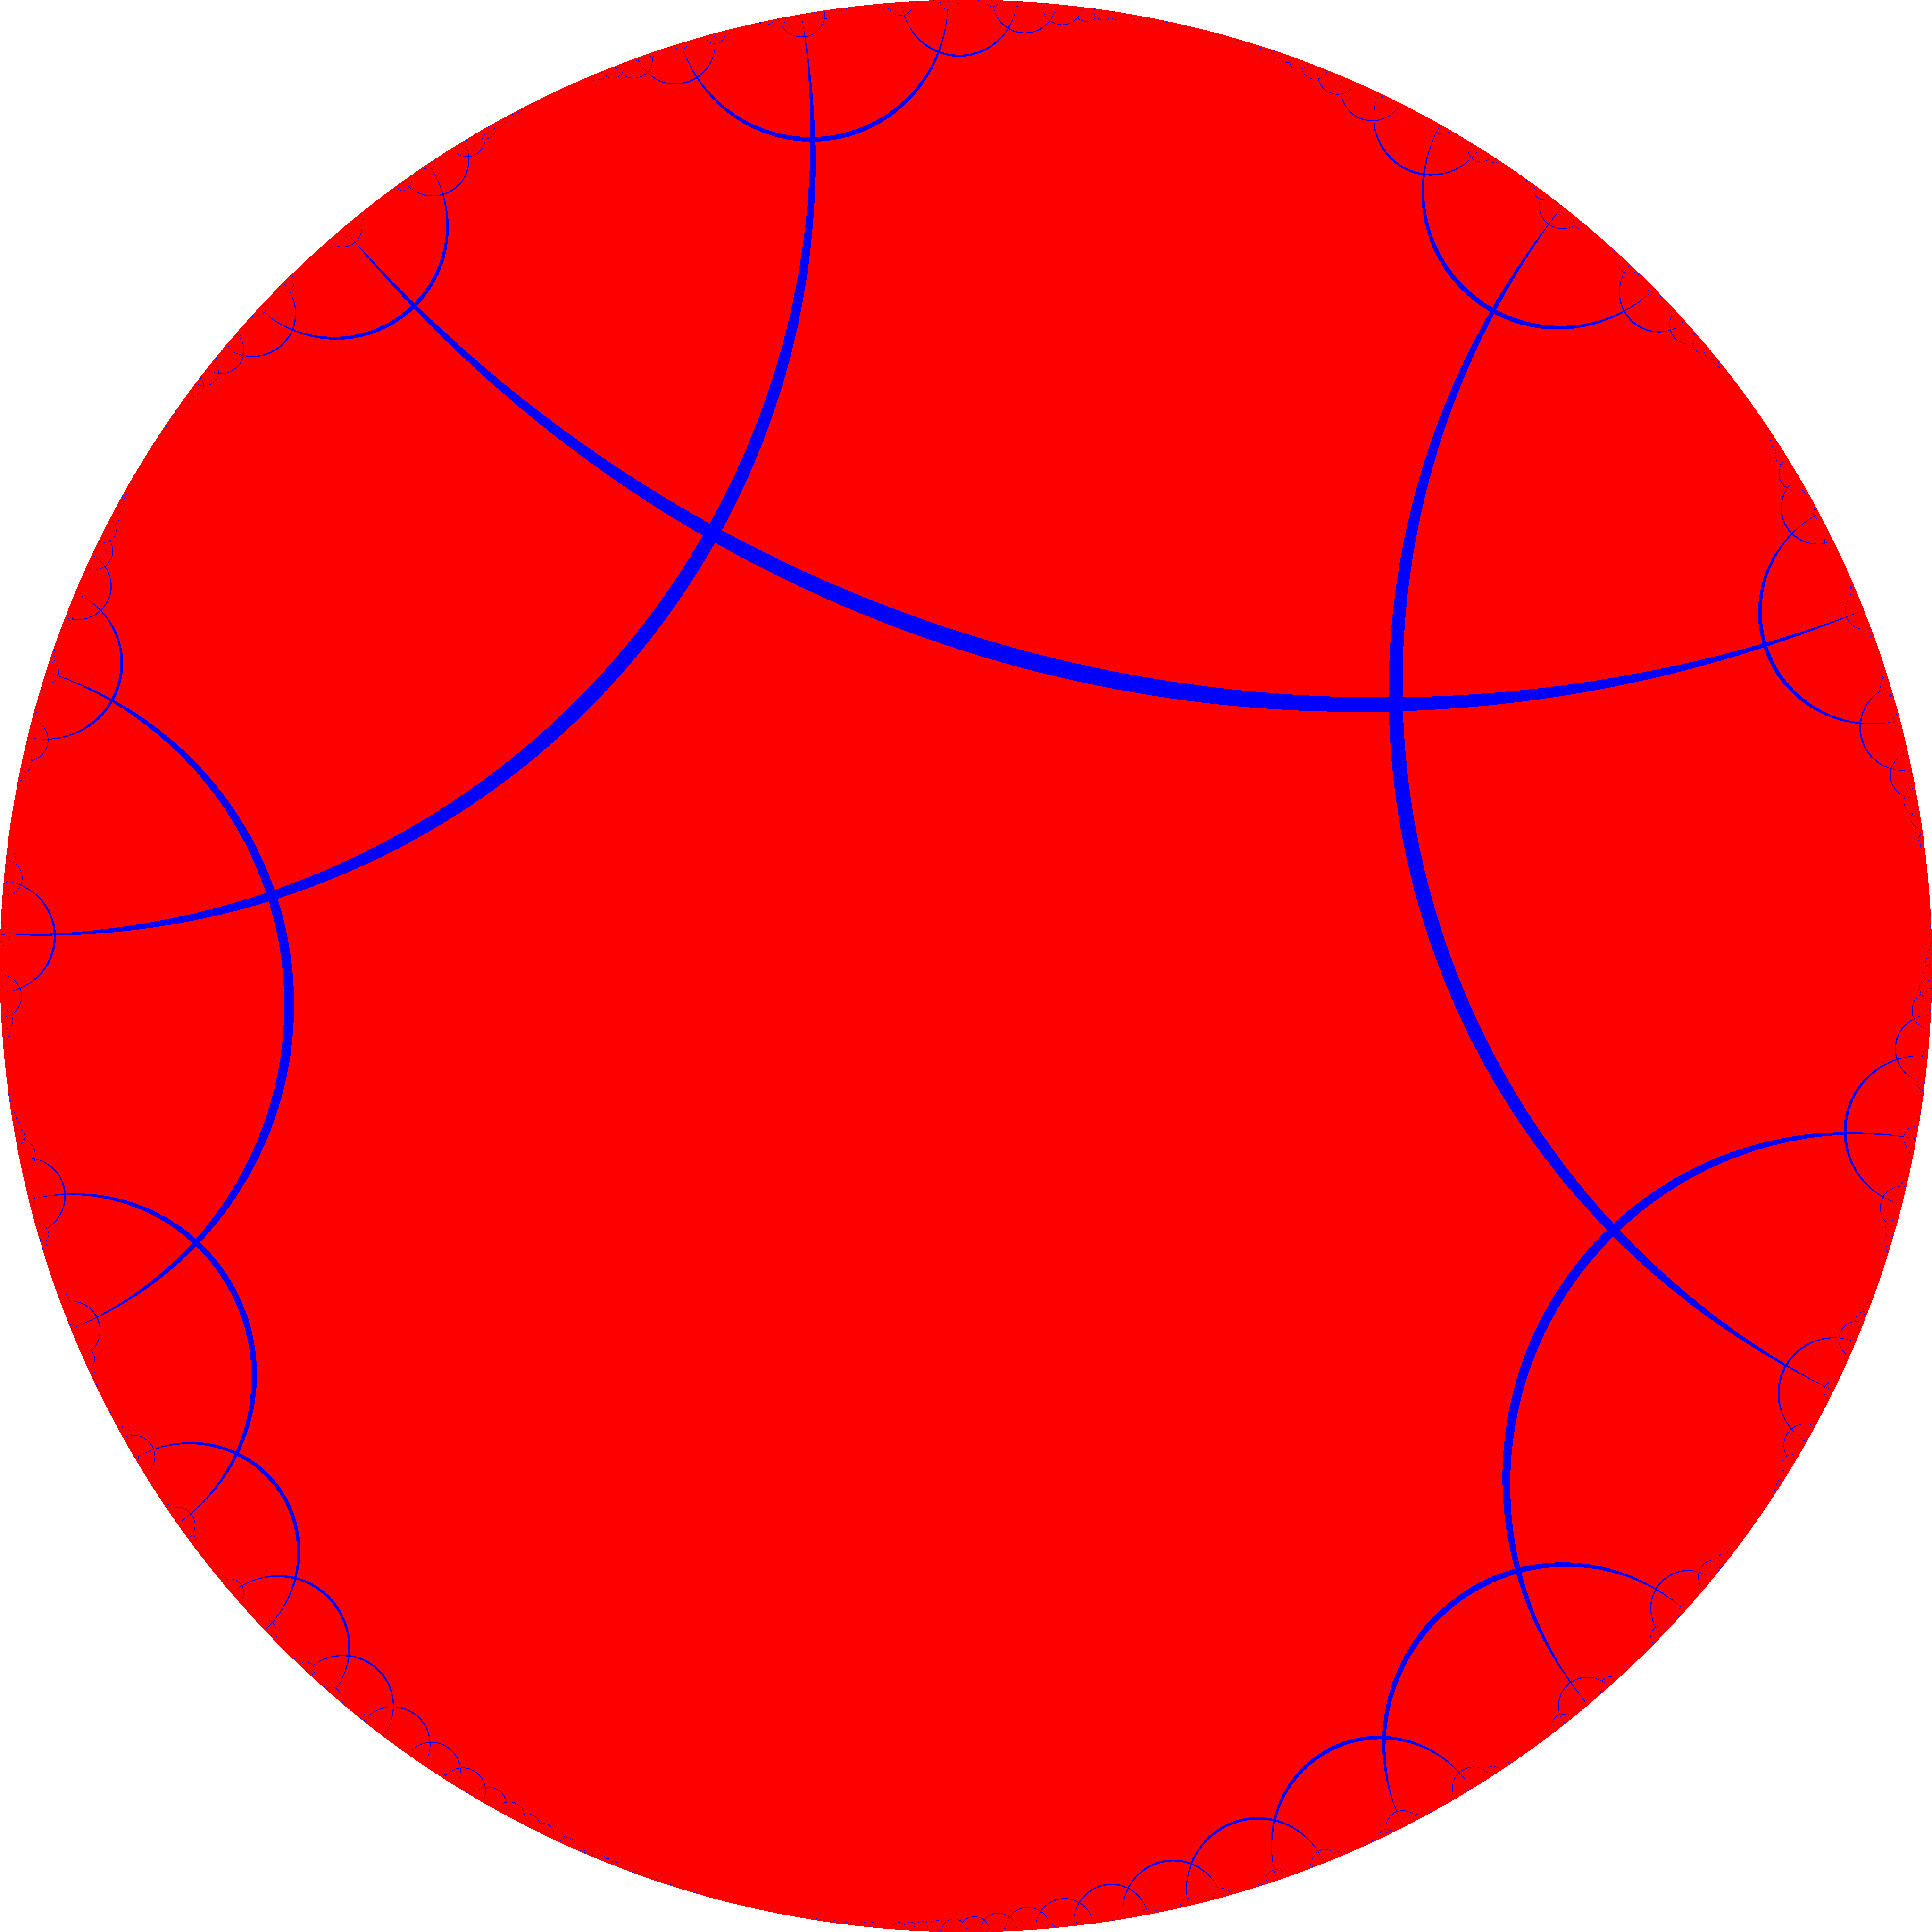
\includegraphics[width=6in]{images/t4096.png}};
    \draw (+0.40, +1.60) node[inner sep=1pt] (g) {$\gamma$};
    \draw (+1.89, +7.89) node[inner sep=1pt] (p_1) {$\infty_1$};
    \draw (-4.29, +6.84) node[inner sep=1pt] (p_2) {$\infty_2$};
    \draw (-7.43, +4.05) node[inner sep=1pt] (p_3) {$\infty_3$};
    \draw (-2.89, -7.89) node[inner sep=1pt] (p_4) {$\infty_4$};
    \draw (+8.58, +0.55) node[inner sep=1pt] (p_5) {$\infty_5$};
    \draw (+6.43, +4.75) node[inner sep=1pt] (p_6) {$\infty_6$};

\end{tikzpicture}
\caption{六个特殊的无穷远点}
\end{figure}

\newpage

\subsubsection{引入镜面映射}

\begin{figure}[ht]
\centering
\begin{tikzpicture}
    \draw (0, 0) node[inner sep=0] {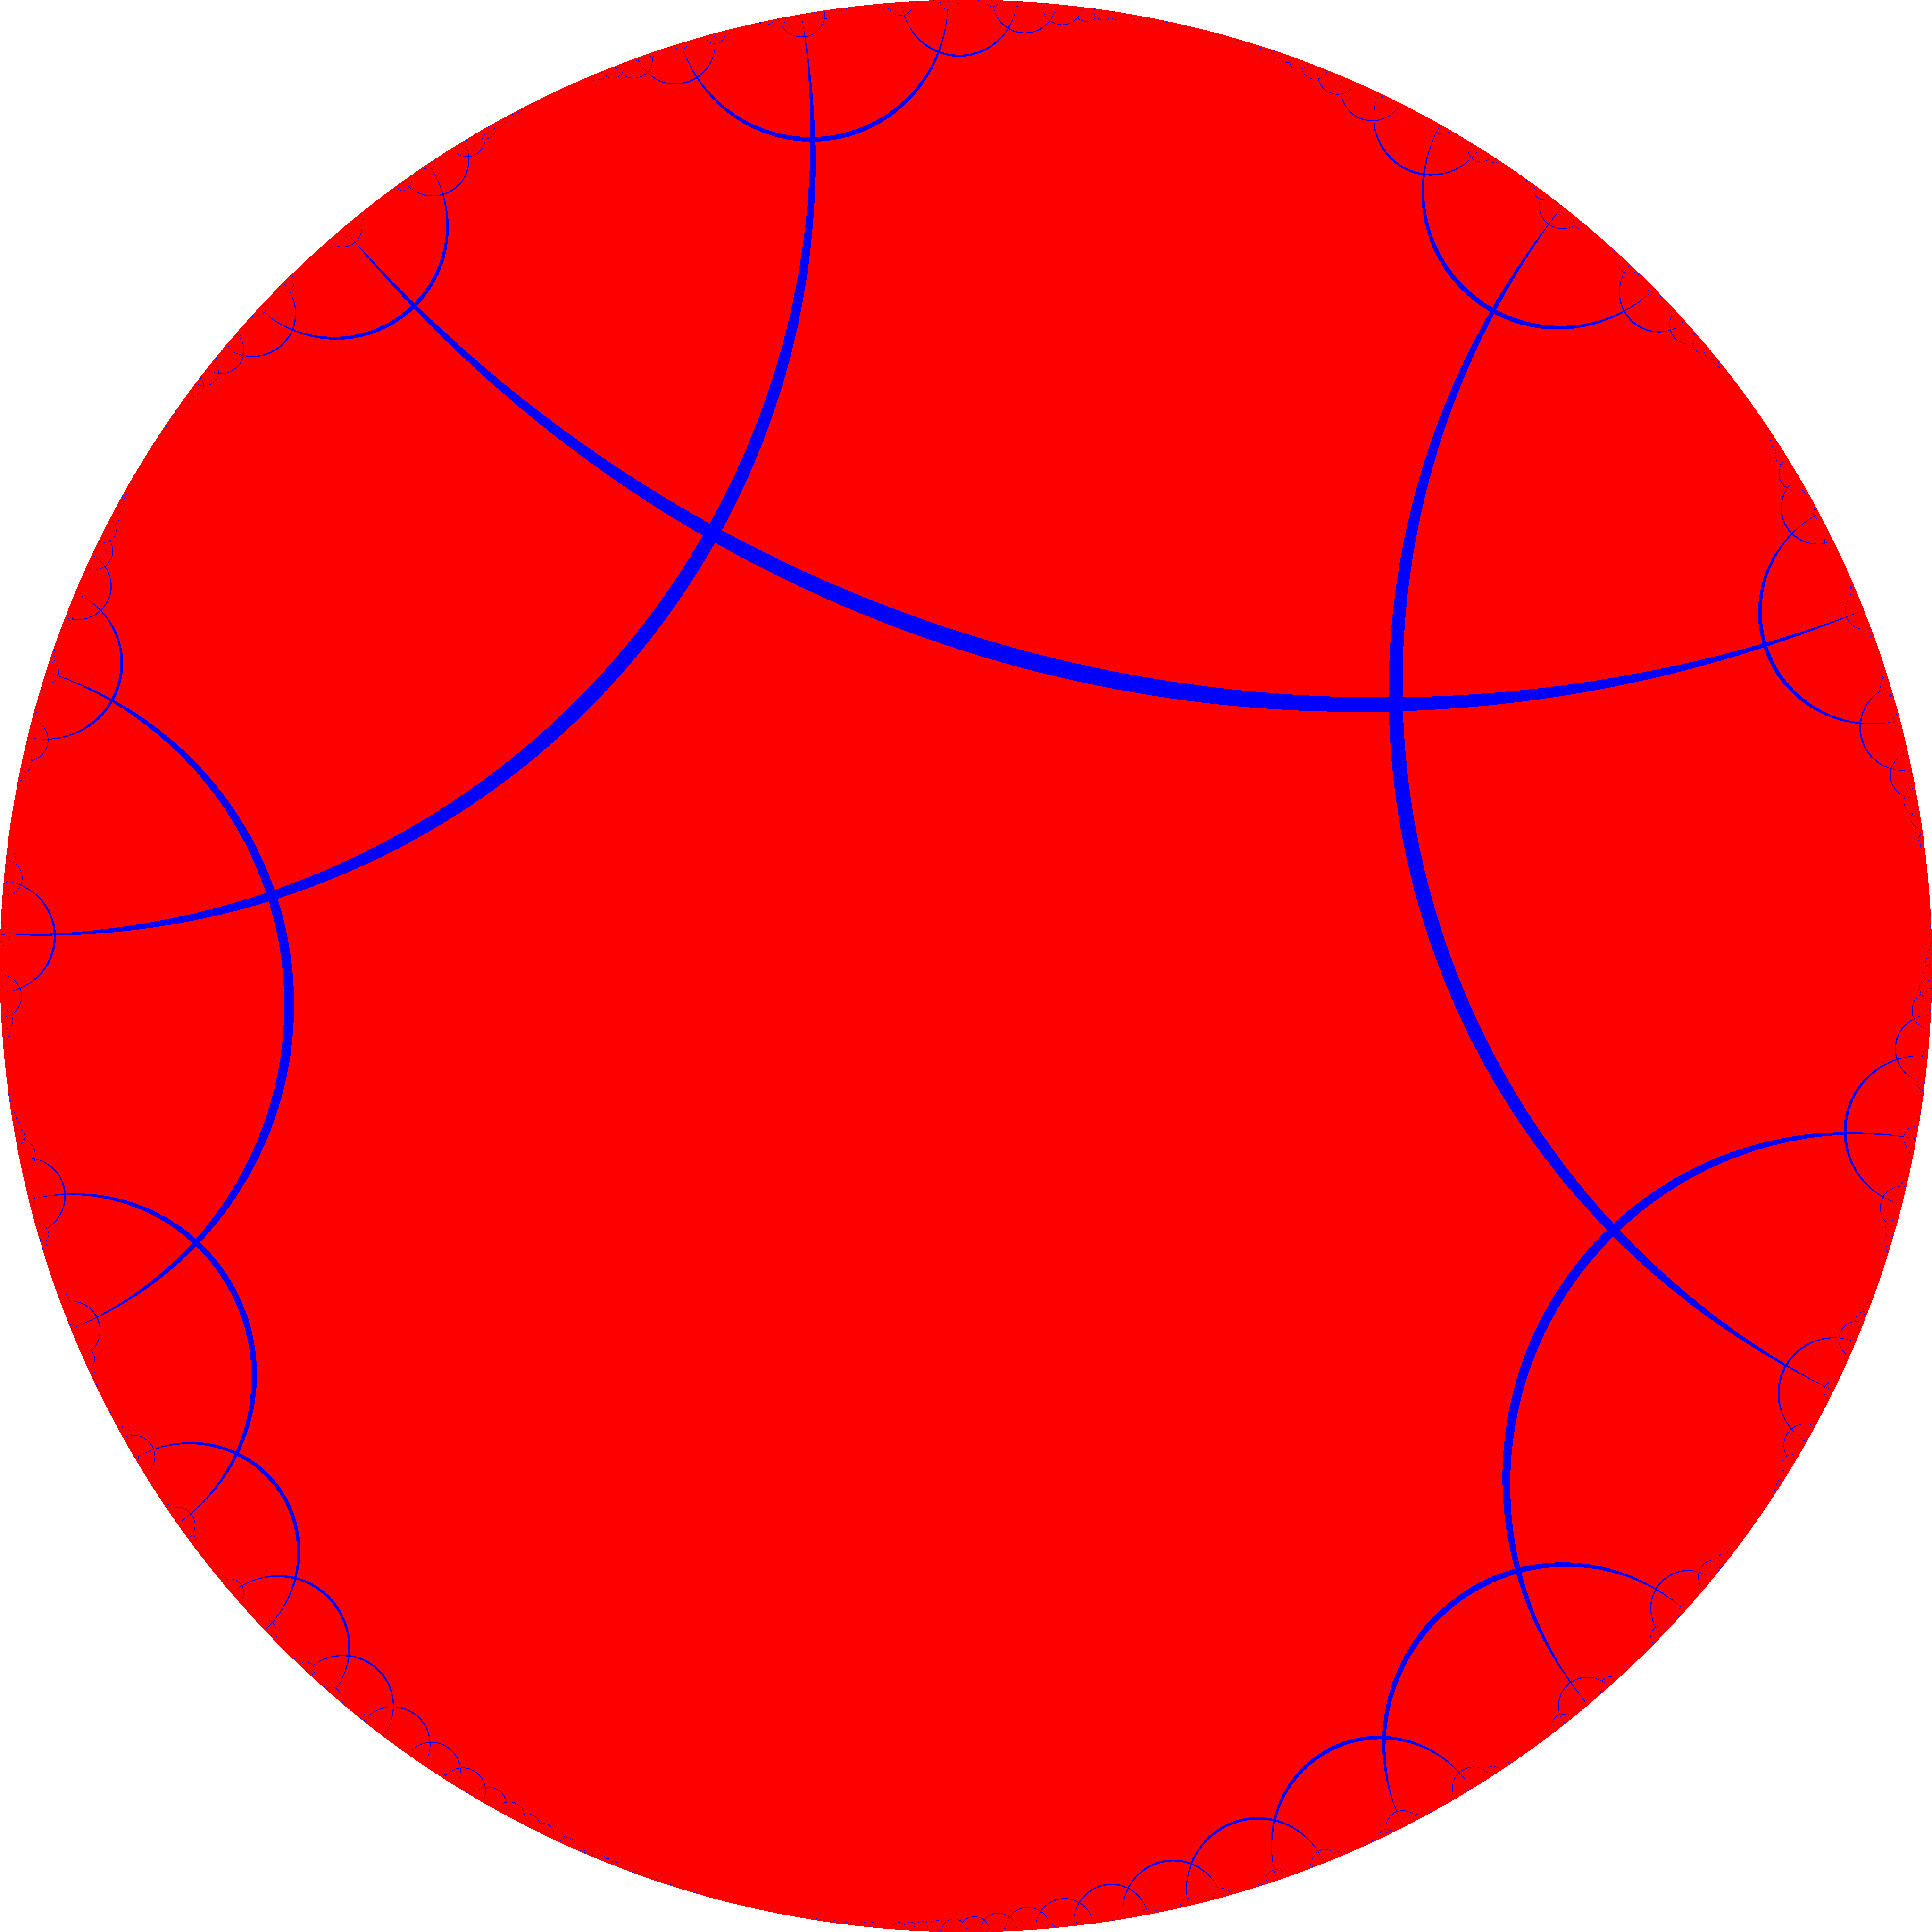
\includegraphics[width=6in]{images/t4096.png}};
    \draw (-4.00, +4.20) node[inner sep=1pt] (g) {$\gamma$};
    \draw (+1.80, +5.20) node[inner sep=1pt] (g_0) {$g_0$};
    \draw (+1.89, +7.89) node[inner sep=1pt] (p_1) {$\infty_1$};
    \draw (-4.29, +6.84) node[inner sep=1pt] (p_2) {$\infty_2$};
    \draw (-7.43, +4.05) node[inner sep=1pt] (p_3) {$\infty_3$};
    \draw (-2.89, -7.89) node[inner sep=1pt] (p_4) {$\infty_4$};
    \draw (+8.58, +0.55) node[inner sep=1pt] (p_5) {$\infty_5$};
    \draw (+6.43, +4.75) node[inner sep=1pt] (p_6) {$\infty_6$};

    \draw [black, dotted, line width=1mm]
          (-1.89, -7.39) node[inner sep=1pt] (p_pinf) {}
       -- (+1.89, +7.39) node[inner sep=1pt] (p_ninf) {};
\end{tikzpicture}
\caption{镜面映射的轴}
\end{figure}

连接 $\infty_1$ 和 $\infty_4$ 得到镜面映射的轴$g_0$。$g_0$是测地线。

\newpage

\subsubsection{沿测地线 $\gamma$ 推移镜面结构}

\begin{figure}[ht]
\centering
\begin{tikzpicture}
    \draw (0, 0) node[inner sep=0] {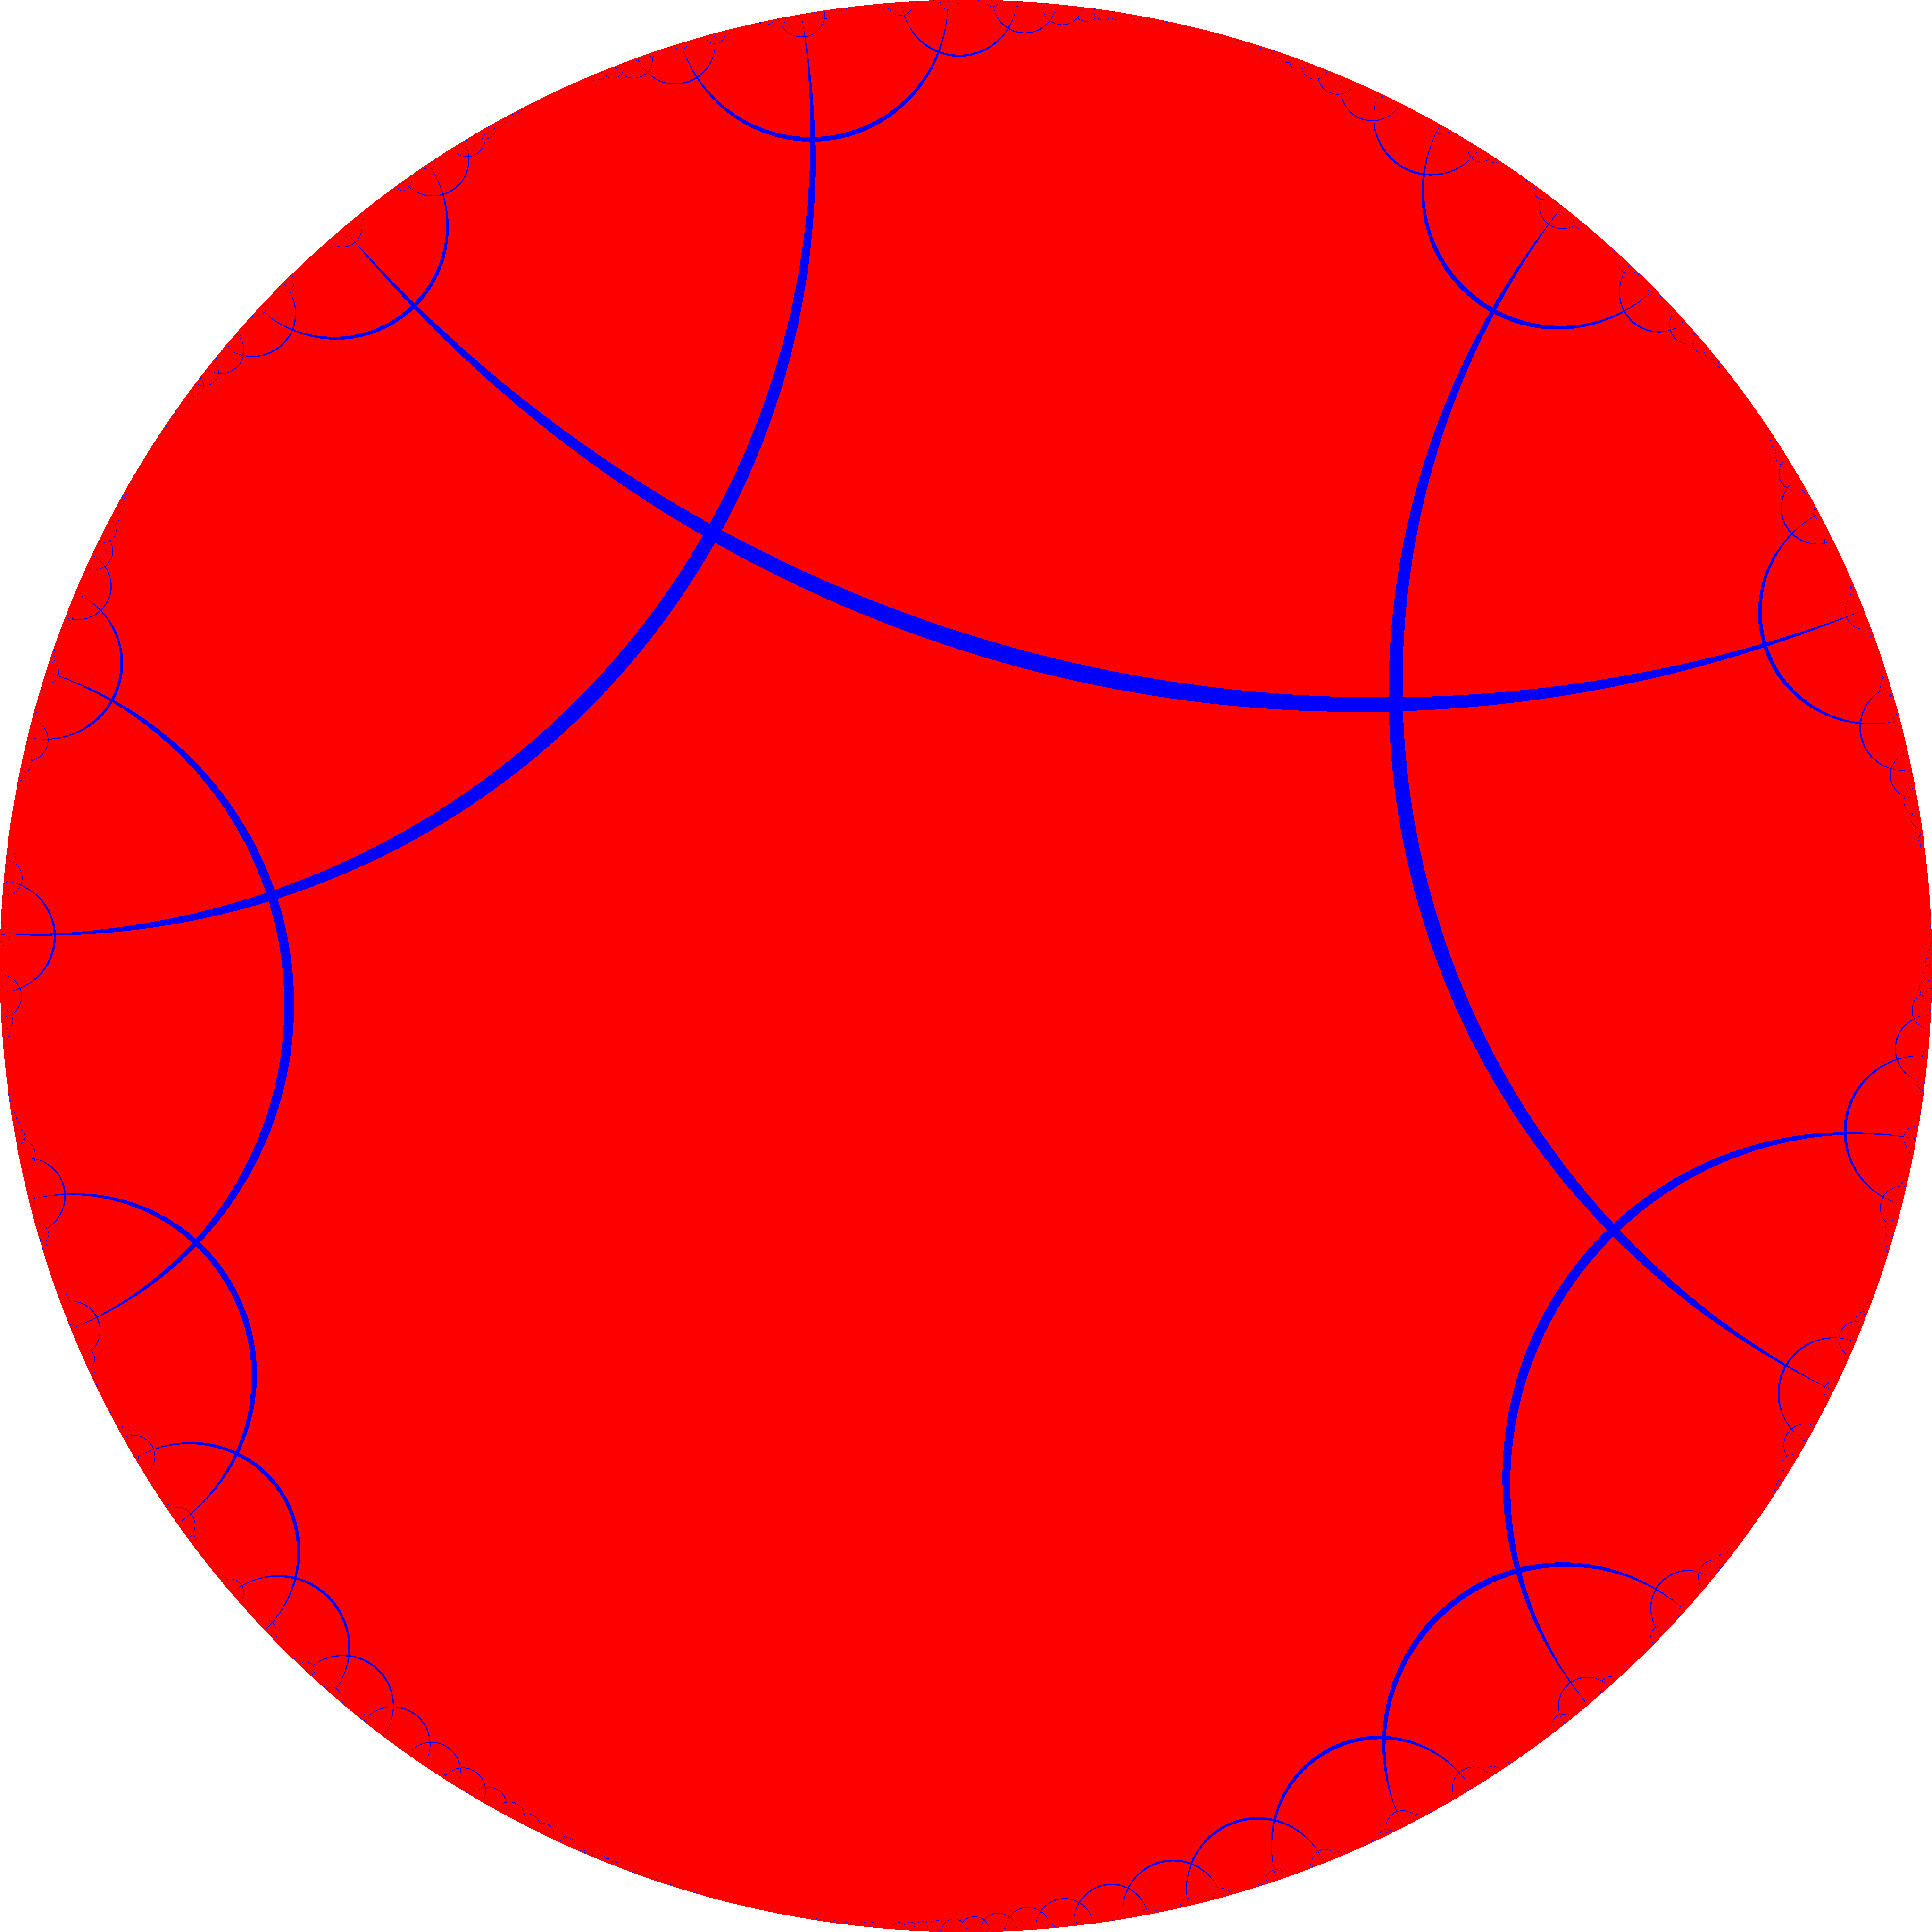
\includegraphics[width=6in]{images/t4096.png}};
    \draw (+1.50, +1.70) node[inner sep=1pt] (g) {$\gamma$};
    \draw (-2.50, +4.70) node[inner sep=1pt] (g_n) {$g_{-1}$};
    \draw (+1.80, +5.20) node[inner sep=1pt] (g_0) {$g_0$};
    \draw (+5.00, +2.80) node[inner sep=1pt] (g_p) {$g_1$};
    \draw (+1.89, +7.89) node[inner sep=1pt] (p_1) {$\infty_1$};
    \draw (-4.29, +6.84) node[inner sep=1pt] (p_2) {$\infty_2$};
    \draw (-7.43, +4.05) node[inner sep=1pt] (p_3) {$\infty_3$};
    \draw (-2.89, -7.89) node[inner sep=1pt] (p_4) {$\infty_4$};
    \draw (+8.58, +0.55) node[inner sep=1pt] (p_5) {$\infty_5$};
    \draw (+6.43, +4.75) node[inner sep=1pt] (p_6) {$\infty_6$};

    % geodesic 0 %
    \draw [black, dotted, line width=1mm]
          (-1.89, -7.39) node[inner sep=1pt] (p_pinf) {}
       -- (+1.89, +7.39) node[inner sep=1pt] (p_ninf) {};

    % geodesic 1 %
    \draw [black, dotted, line width=1mm]
          (-3.29, 6.84) arc (205.0:58.7:-2.20);

    % line 0 %
    \draw [green, dotted, thick]
          (-3.29, 6.84) arc (240:271.7:18.00);

    % geodesic 1 %
    \draw [black, dotted, line width=1mm]
          (7.58, 0.55) arc (265.0:135.7:2.25);

   % line 1 %
    \draw [green, dotted, thick]
          (-6.43, 4.05) arc (240:271.7:26.50);

\end{tikzpicture}
\caption{沿测地线 $\gamma$ 推移镜面结构}
\end{figure}

\newpage

\subsection{Surreal数}

\begin{figure}[ht]
\centering
\begin{tikzpicture}
    \draw (0, 0) node[inner sep=0] {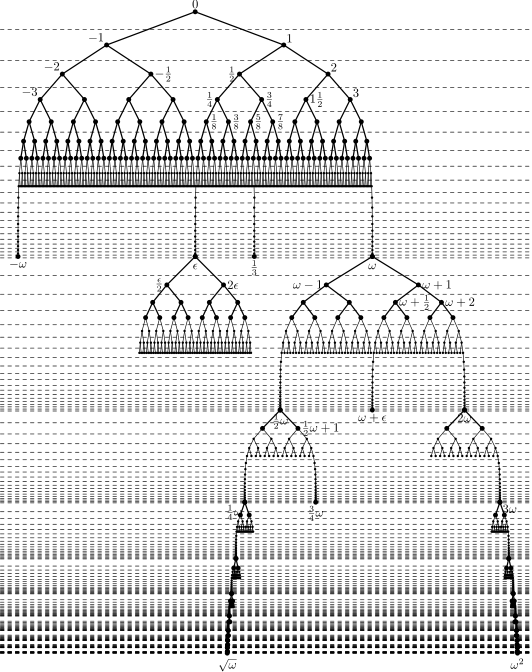
\includegraphics[width=4in]{images/surreal.png}};
\end{tikzpicture}
\caption{Surreal数的生成树}
\end{figure}

Surreal数按照生成树的先序遍历是严格从小到大的。Surreal数是一种序和代数的结构,有非常强大的序关系。

\newpage

\section{共形嵌入的想法}

Surreal数的生成树具有高度的规律性,我们猜测Surreal数的生成树可以嵌入到加乘树里面,而且每个树枝都是一条测地线。

\subsection{嵌入$0$}

\begin{figure}[ht]
\centering
\begin{tikzpicture}
    \draw (0, 0) node[inner sep=0] {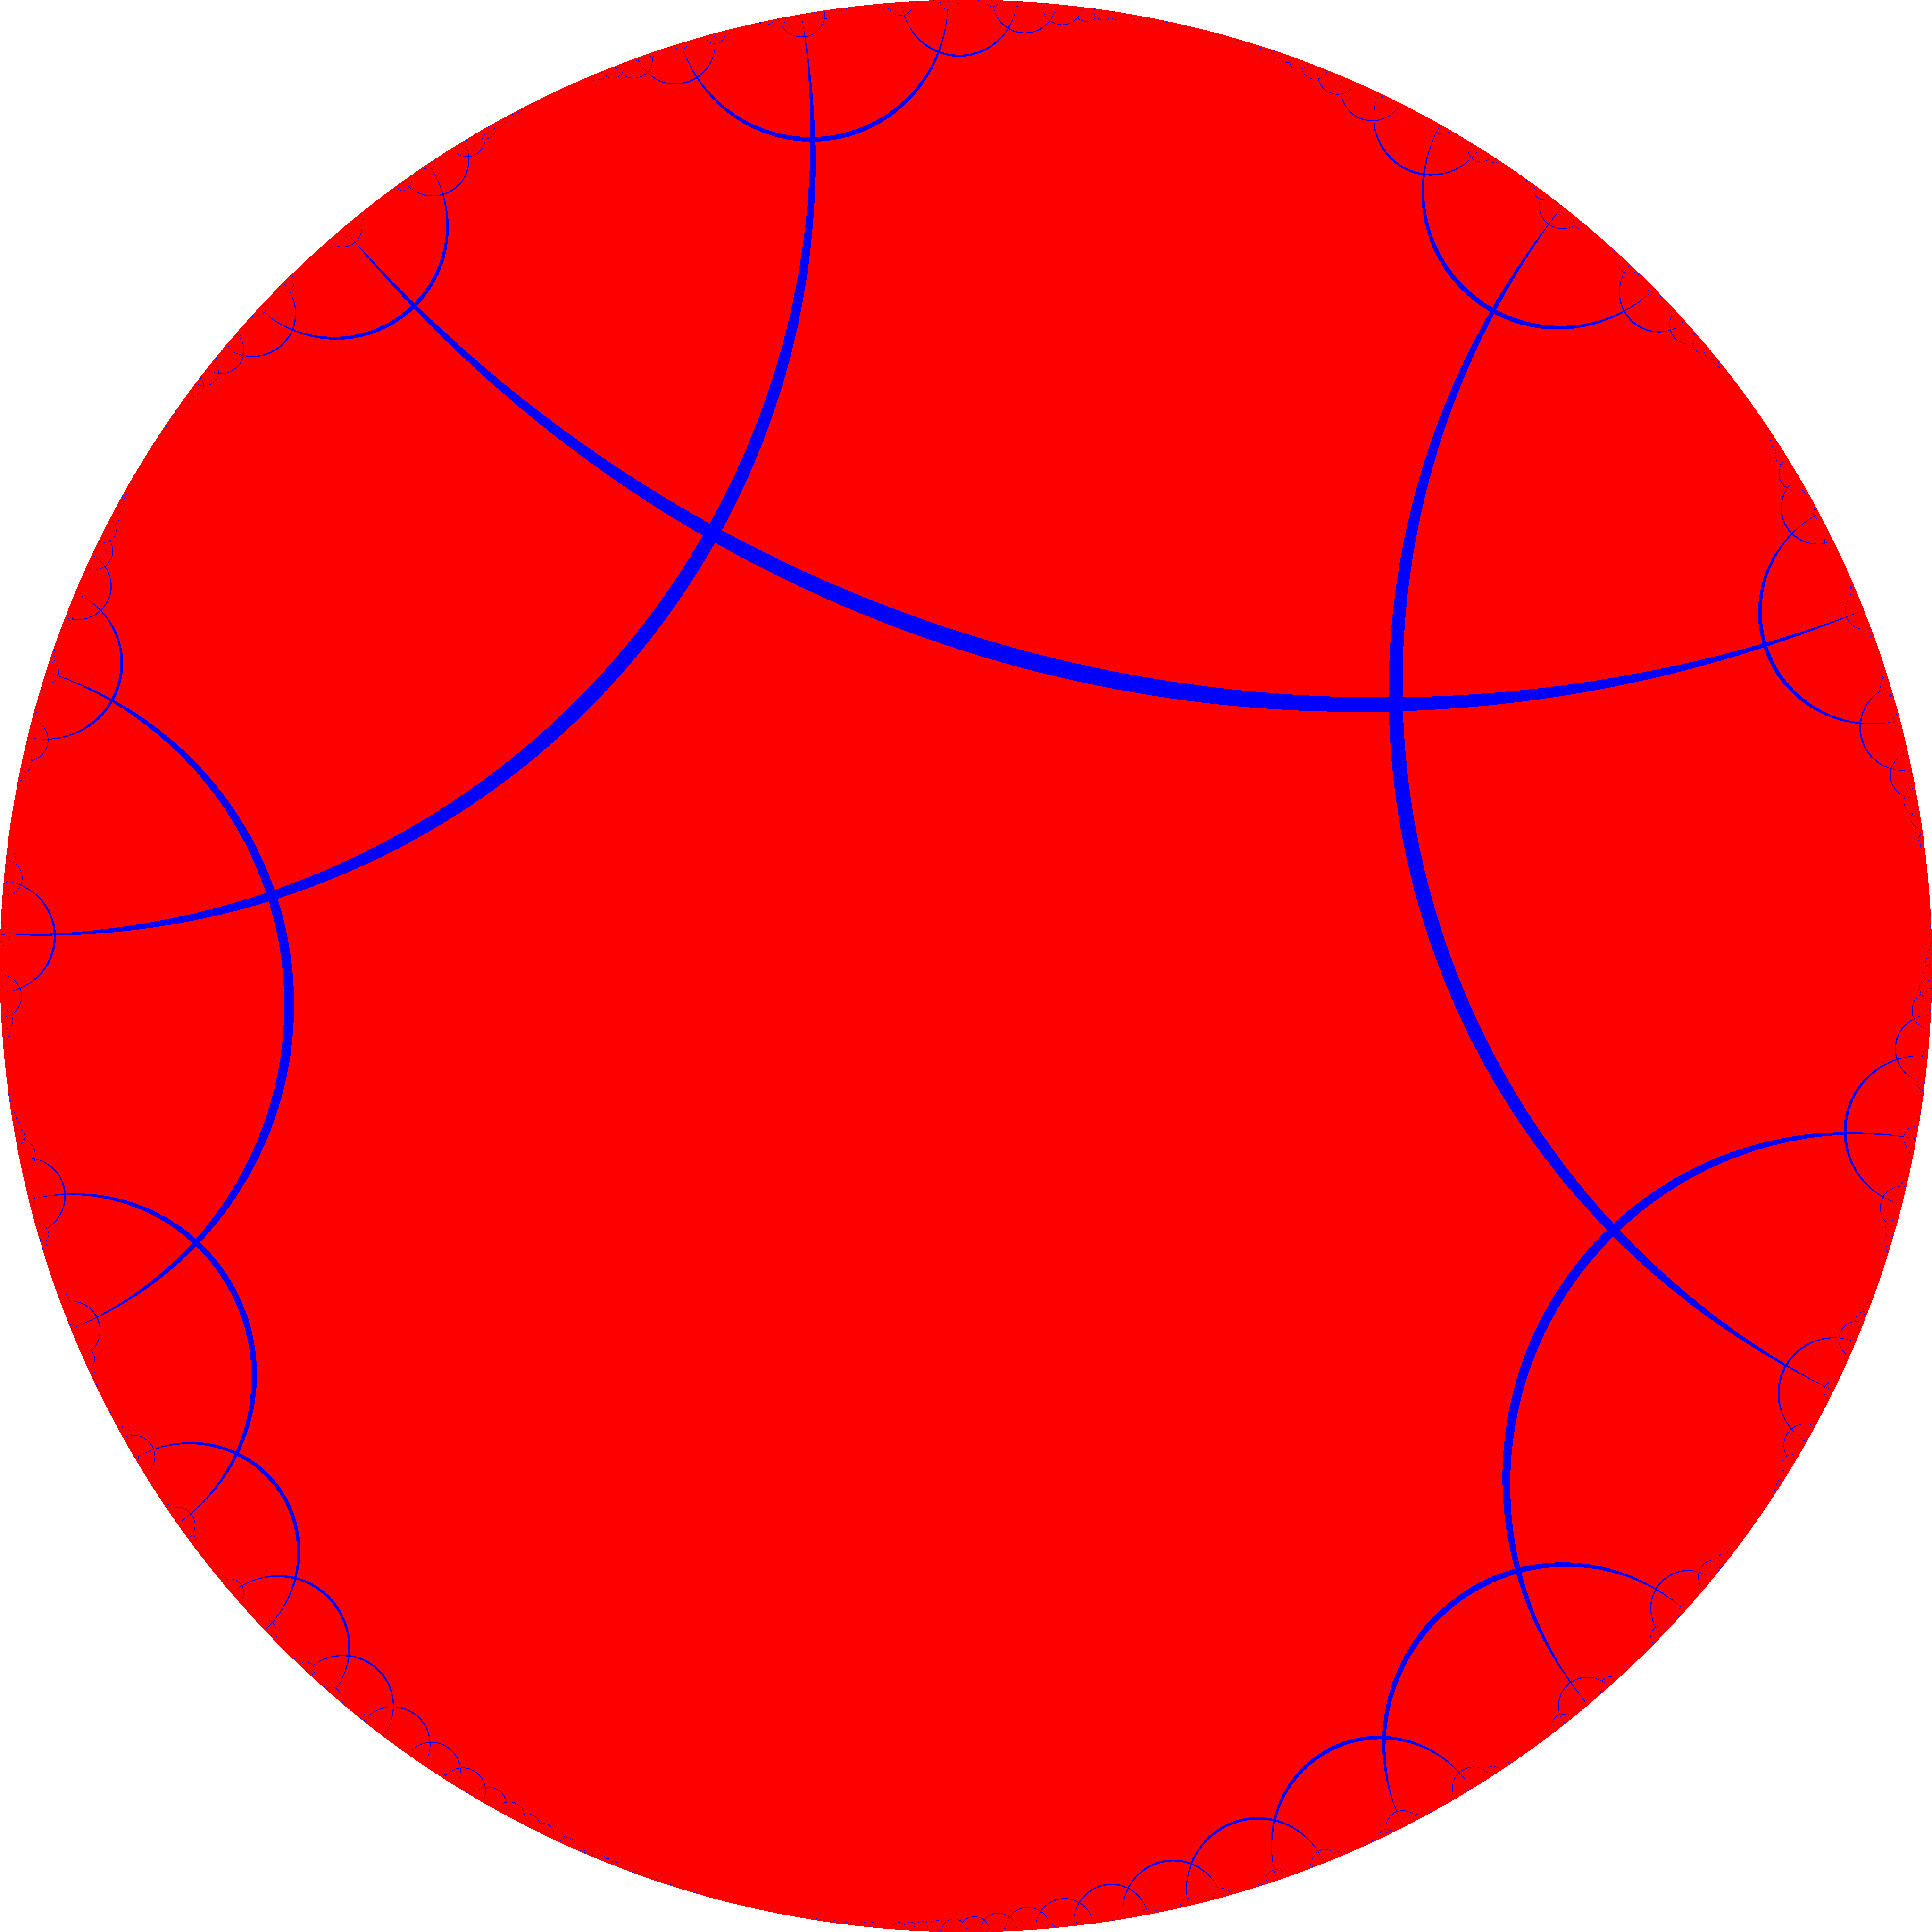
\includegraphics[width=6in]{images/t4096.png}};
    \draw (-1.35, -3.50) node[inner sep=1pt] (p_z) {0};

    % geodesic 0 %
    \draw [black, dotted, line width=0.3mm]
          (-1.89, -7.39) node[inner sep=1pt] (p_pinf) {}
       -- (+1.89, +7.39) node[inner sep=1pt] (p_ninf) {};

    \draw (-0.9, +6.2) node {$-1$};
    \draw (-1.9, +2.9) node {$-\frac{1}{2}$};
    \draw (-5.0, +0.3) node {$-\frac{1}{4}$};
    \draw (-7.0, +0.0) node {$-\frac{1}{8}$};

    \draw (+3.7, +4.9) node {$+1$};
    \draw (+3.1, +1.7) node {$+\frac{1}{2}$};
    \draw (+5.2, -2.5) node {$+\frac{1}{4}$};
\end{tikzpicture}
\caption{嵌入$0$ 线}
\end{figure}

\newpage

\subsection{嵌入$n$}

\begin{figure}[ht]
\centering
\begin{tikzpicture}
    \draw (0, 0) node[inner sep=0] {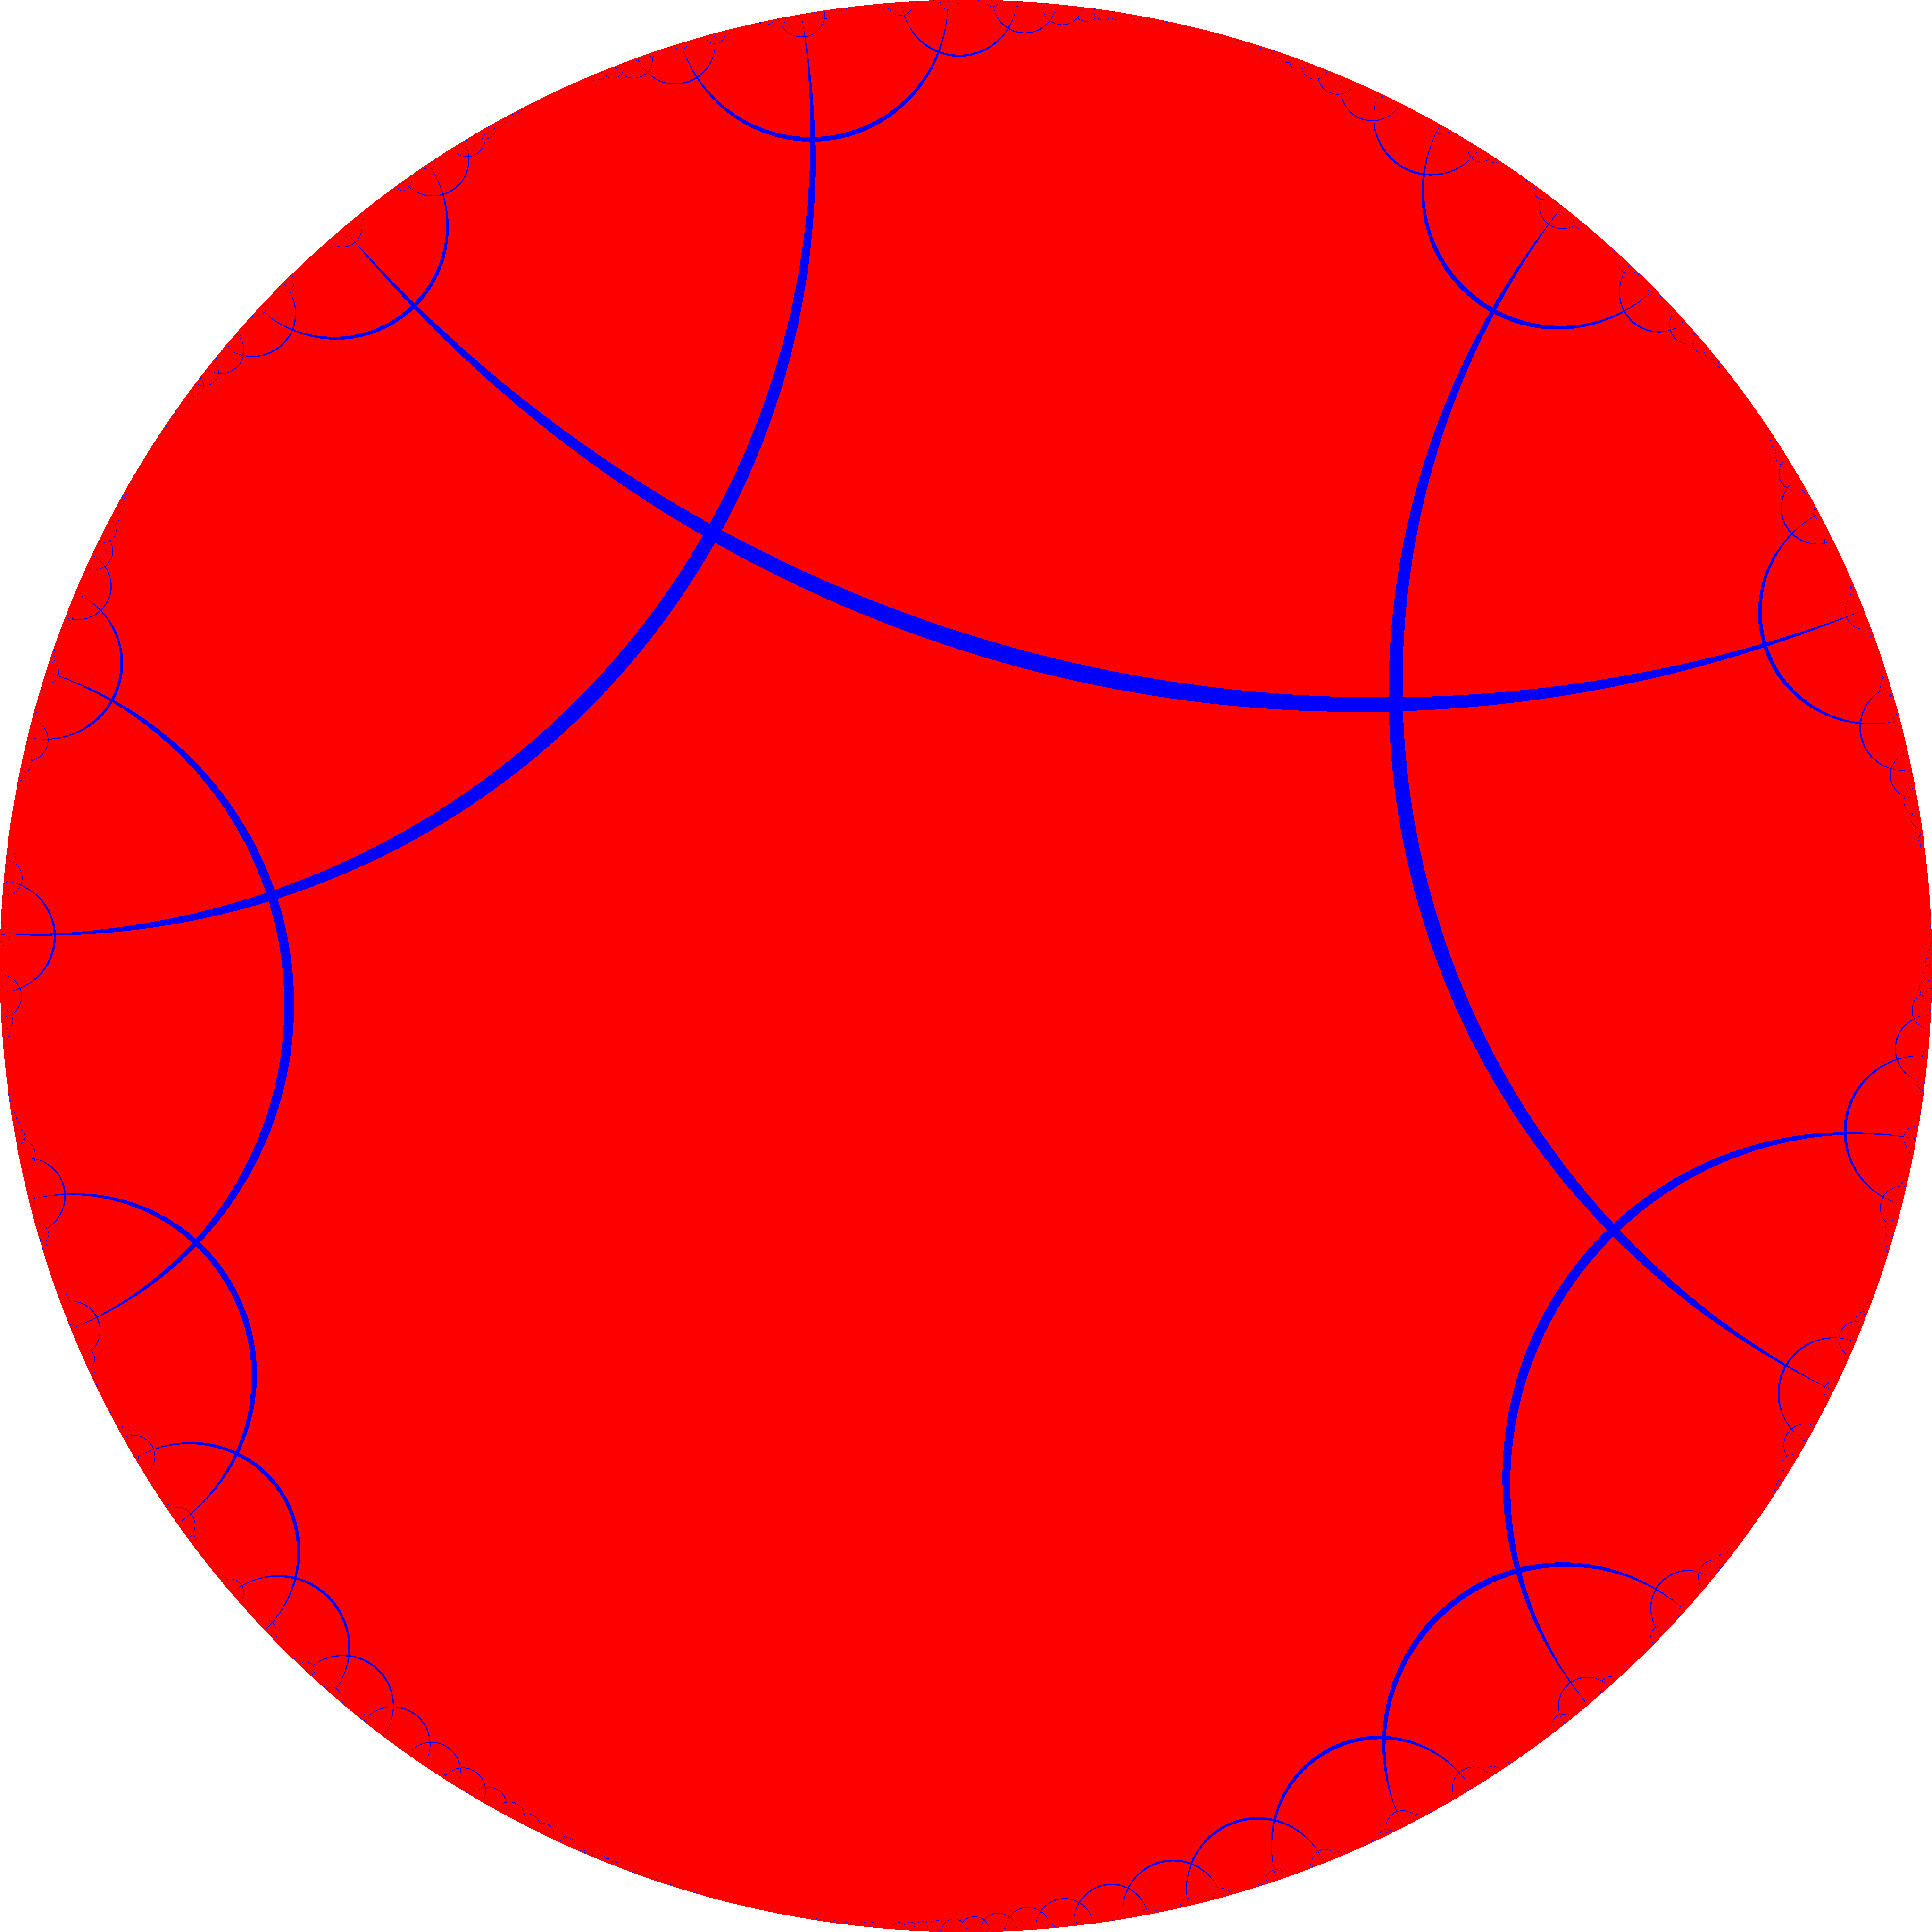
\includegraphics[width=6in]{images/t4096.png}};
    \draw (1.00, 2.60) node[inner sep=1pt] (p_z) {0};
    \draw (-3.4, +3.9) node {$-1$};
    \draw (+5.2, +1.8) node {$+1$};

    % geodesic 0 %
    \draw [black, dotted, line width=1mm]
          (-1.89, -7.39) node[inner sep=1pt] (p_pinf) {}
       -- (+1.89, +7.39) node[inner sep=1pt] (p_ninf) {};

    % geodesic 1 %
    \draw [black, dotted, line width=1mm]
          (-3.29, 6.84) arc (205.0:58.7:-2.20);

    % geodesic 1 %
    \draw [black, dotted, line width=1mm]
          (7.58, 0.55) arc (265.0:135.7:2.25);

    \draw (-0.9, +6.2) node {$-1$};
    \draw (-1.9, +2.9) node {$-\frac{1}{2}$};
    \draw (-5.0, +0.3) node {$-\frac{1}{4}$};
    \draw (-7.0, +0.0) node {$-\frac{1}{8}$};

    \draw (+3.7, +4.9) node {$+1$};
    \draw (+3.1, +1.7) node {$+\frac{1}{2}$};
    \draw (+5.2, -2.5) node {$+\frac{1}{4}$};
\end{tikzpicture}
\caption{嵌入 $n$ 线}
\end{figure}

\newpage

\subsection{嵌入$2^{-n}$}

为了看到所有的 $2^{-n}$,我们把上图中的观察视角左移 $\frac{1}{2}$,于是黑枝变成蓝枝,就能看到所有的 $2^{-n}$ 分布在右侧的蓝主枝上。

\begin{figure}[ht]
\centering
\begin{tikzpicture}
    \draw (0, 0) node[inner sep=0] {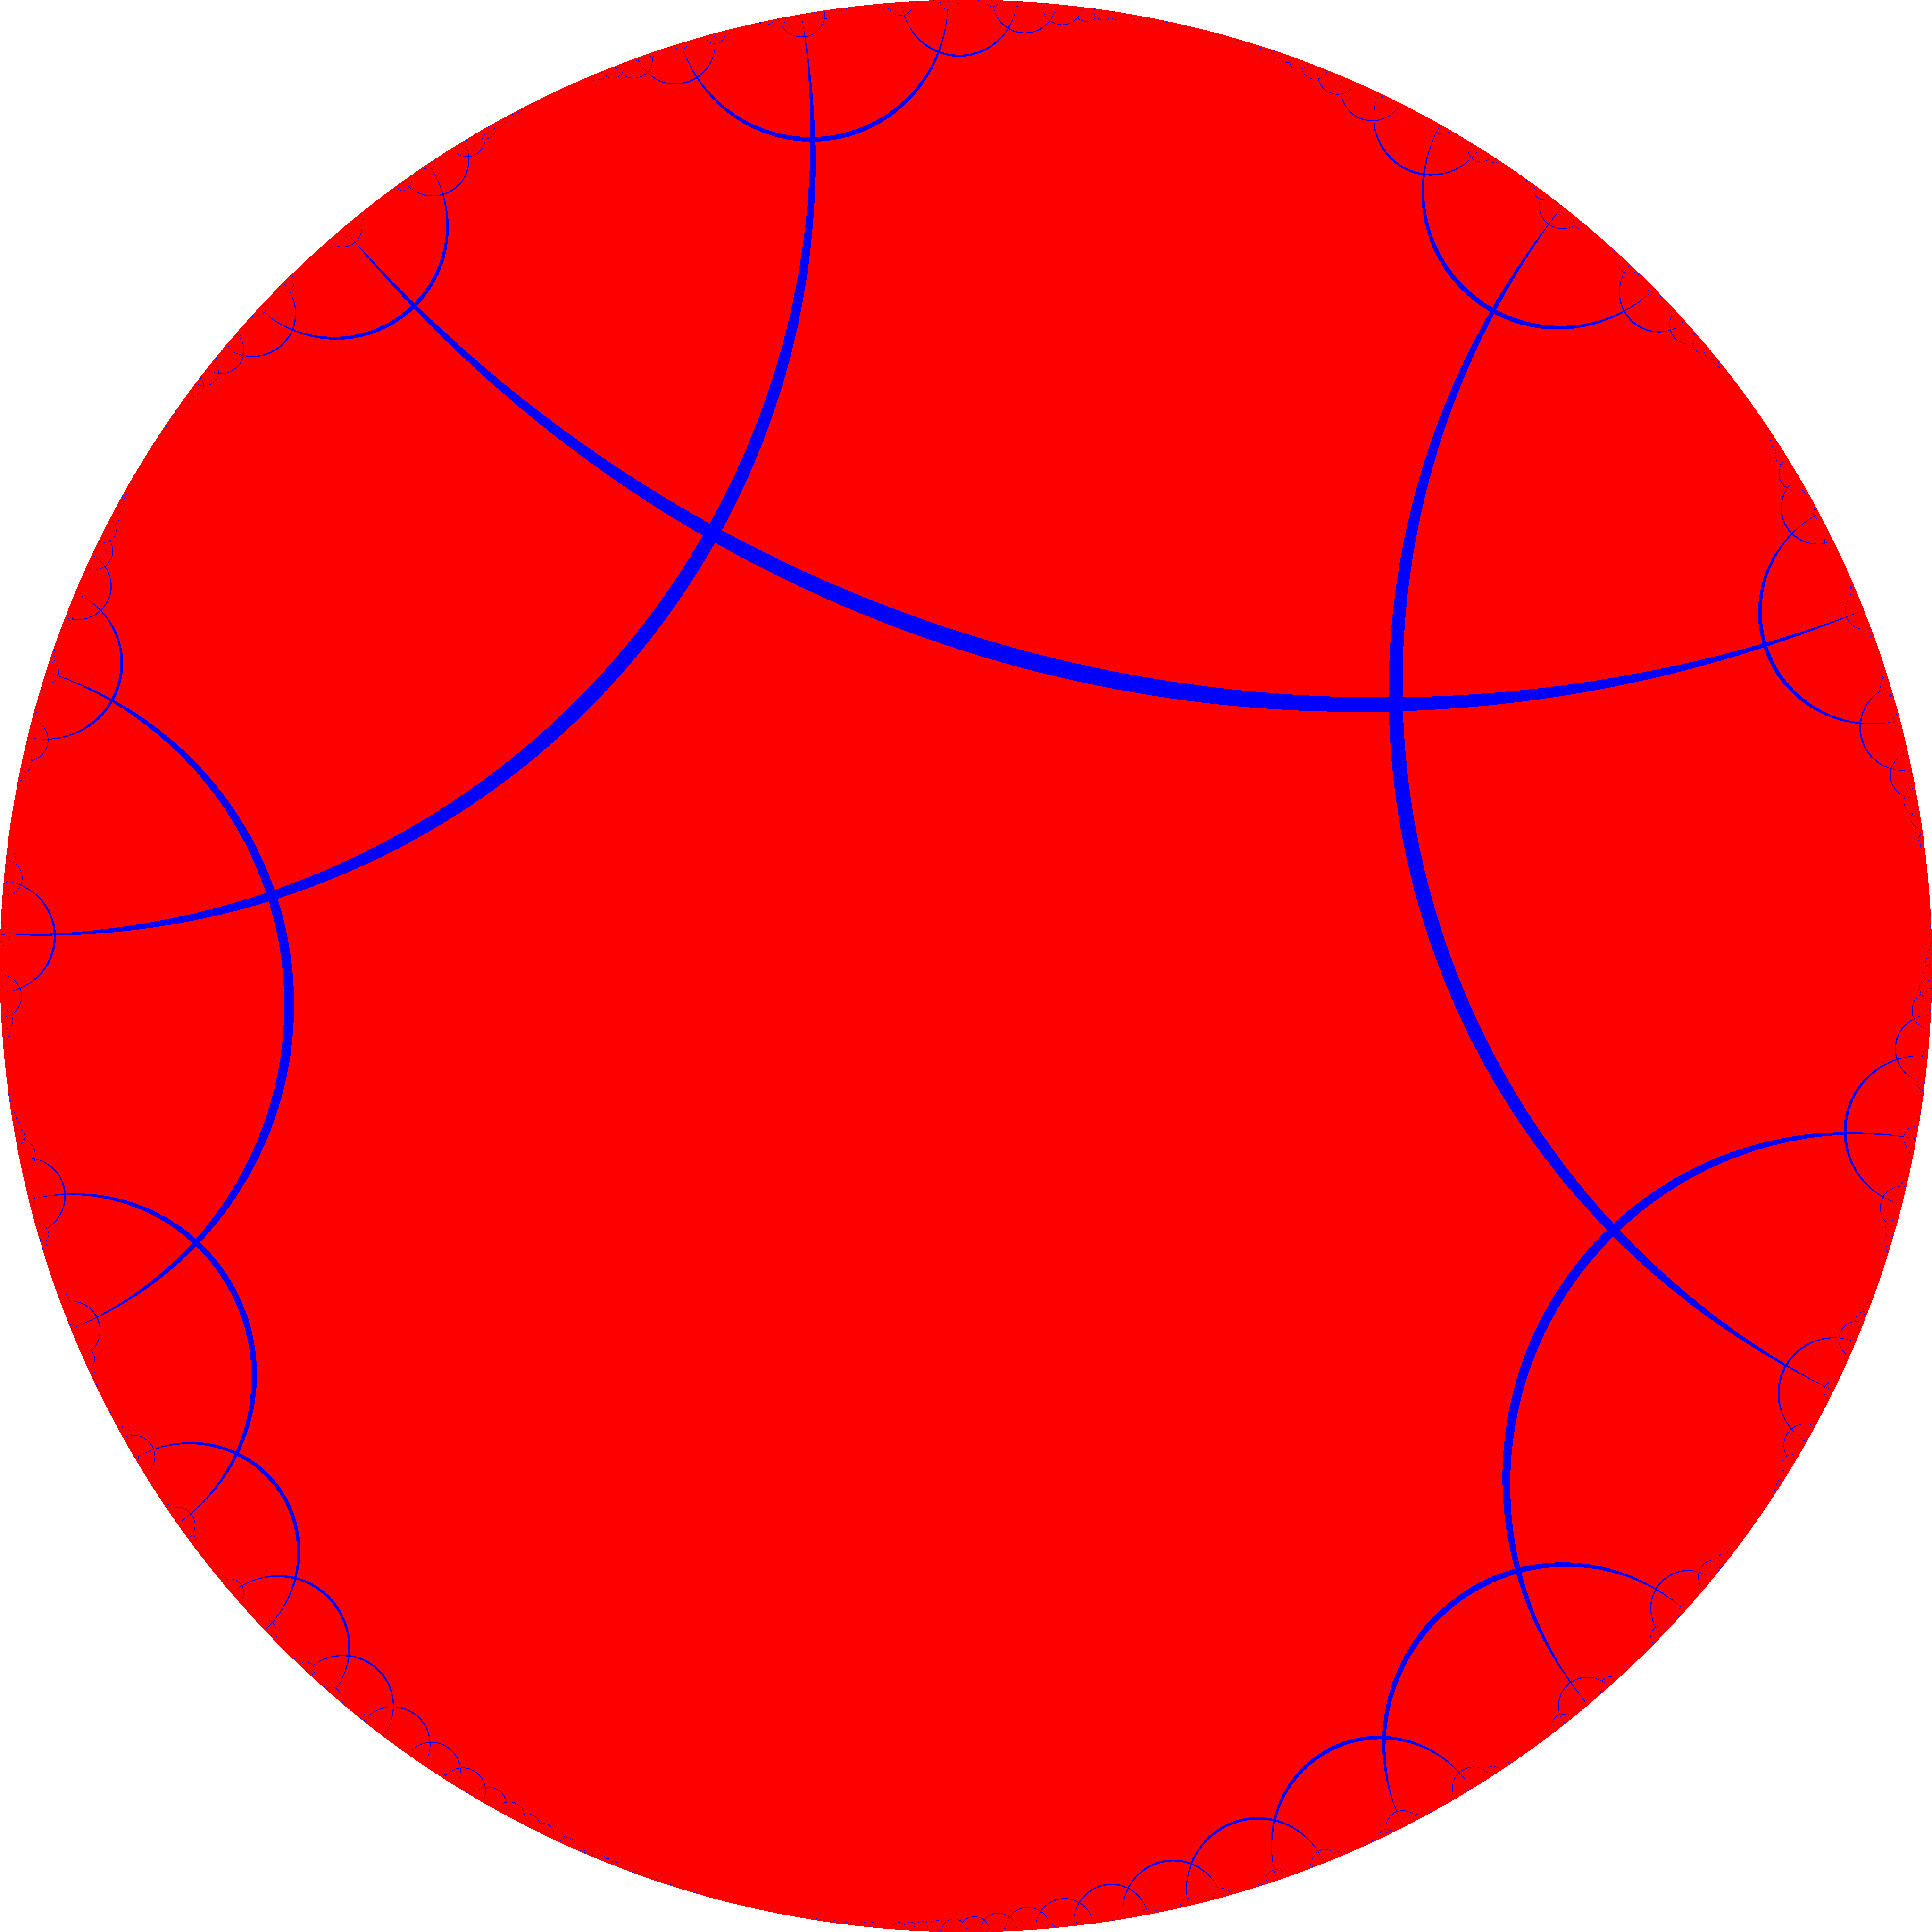
\includegraphics[width=6in]{images/t4096.png}};
    \draw (1.00, 2.60) node[inner sep=1pt] (p_z) {$+\frac{1}{2}$};
    \draw (-3.4, +3.9) node {$-\frac{1}{2}$};
    \draw (+5.2, +1.8) node {$+\frac{3}{2}$};

    \draw (-0.9, +6.2) node {$+0$};
    \draw (-1.9, +2.9) node {$+0$};
    \draw (-5.0, +0.3) node {$+0$};
    \draw (-7.0, +0.0) node {$+0$};

    \draw (+3.7, +4.9) node {$+2$};
    \draw (+3.1, +1.7) node {$+1$};
    \draw (+5.2, -2.5) node {$+\frac{1}{2}$};

    \draw (+0.00, +0.00) node {$+\frac{1}{4}$};

    % geodesic 0 %
    \draw [black, dotted, line width=1mm]
          (-1.89, -7.39) node[inner sep=1pt] (p_pinf) {}
       -- (+1.89, +7.39) node[inner sep=1pt] (p_ninf) {};

    % geodesic 1 %
    \draw [black, dotted, line width=1mm]
          (-3.29, 6.84) arc (205.0:58.7:-2.20);

    % line 0 %
    \draw [green, dotted, thick]
          (-3.29, 6.84) arc (240:271.7:18.00);

    % geodesic 1 %
    \draw [black, dotted, line width=1mm]
          (7.58, 0.55) arc (265.0:135.7:2.25);

    % line 0 %
    \draw [green, dotted, thick]
          (-3.29, 6.84) arc (240:271.7:18.00);

   % line 1 %
    \draw [green, dotted, thick]
          (-6.43, 4.05) arc (240:271.7:26.50);

   % line 2 %
    \draw [green, dotted, thick]
          (6.30, -4.30) arc (240:272.7:-25.50);

   % line 3 %
    \draw [green, dotted, thick]
          (4.38, -6.15) arc (240:273.0:-20.30);
\end{tikzpicture}
\caption{嵌入$2^{-n}$}
\end{figure}

\newpage

\subsection{嵌入$1 - 2^{-n}$}

为了看到所有的 $1 - 2^{-n}$,我们把上图中的观察视角再左移 $1$,$1 - 2^{-n}$ 出现在图中,并分布在一条特殊的枝上。

\begin{figure}[ht]
\centering
\begin{tikzpicture}
    \draw (0, 0) node[inner sep=0] {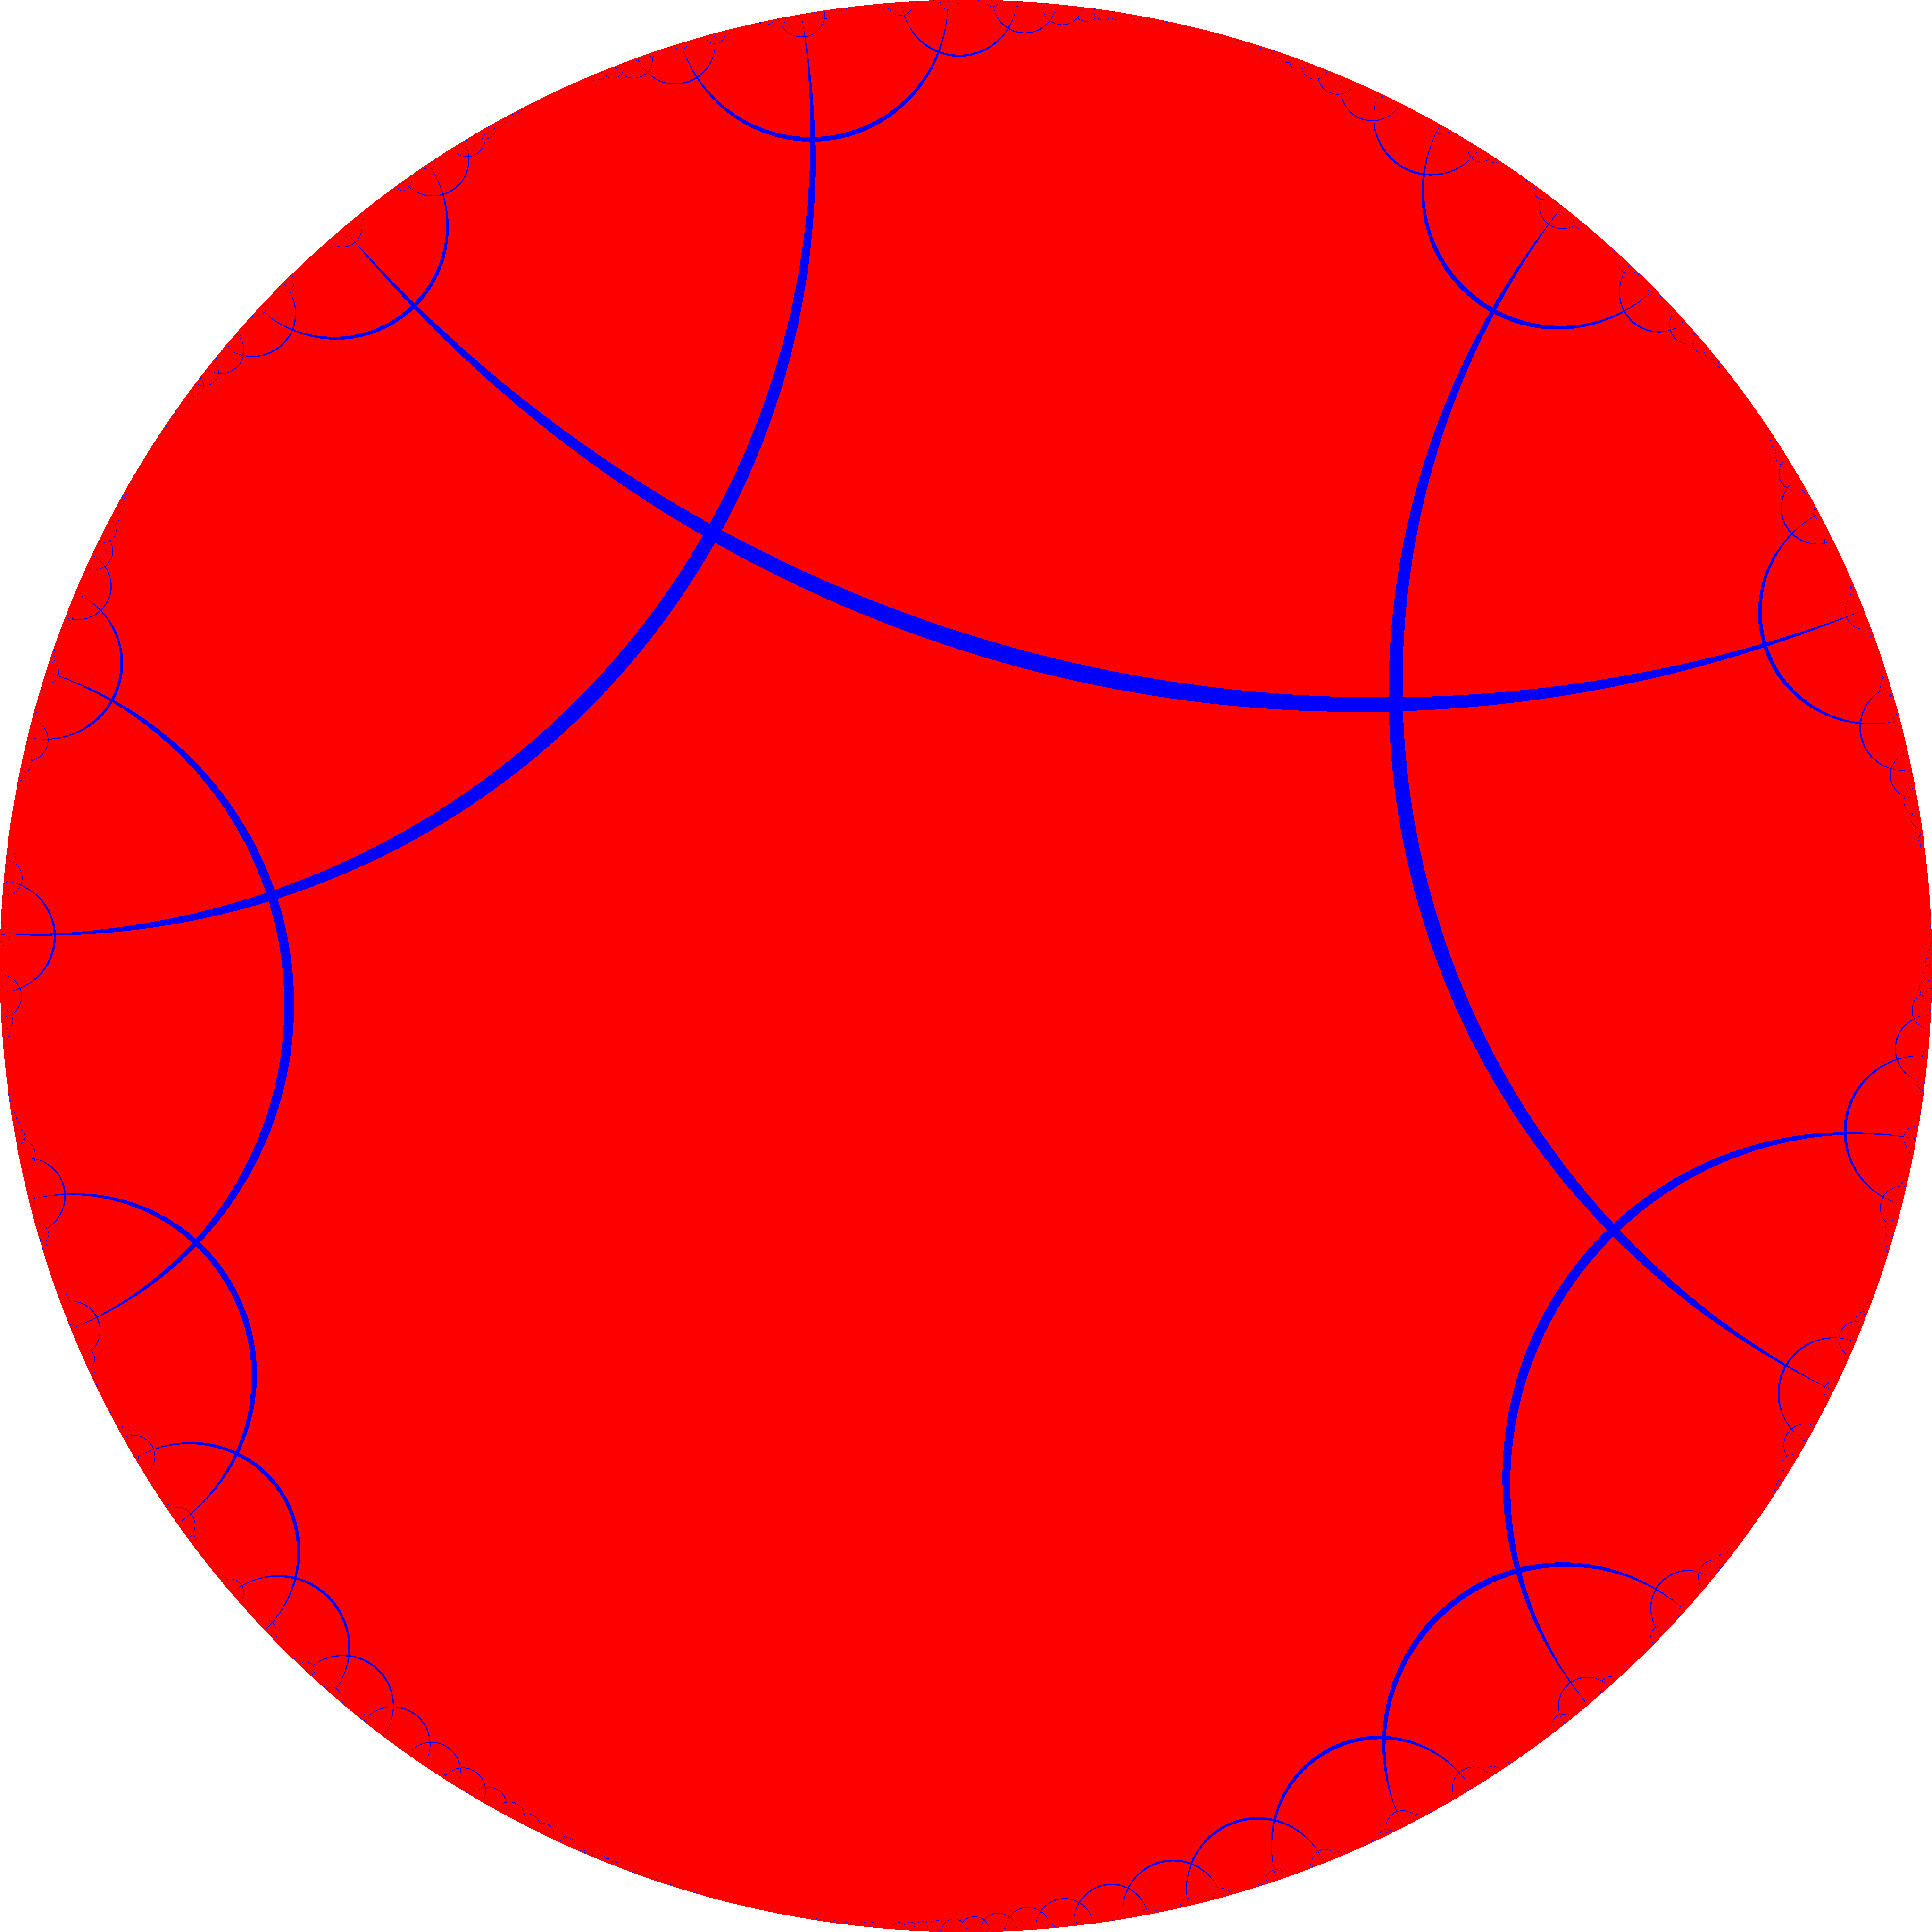
\includegraphics[width=6in]{images/t4096.png}};
    \draw (1.00, 2.60) node[inner sep=1pt] (p_z) {$+\frac{3}{2}$};
    \draw (-3.4, +3.9) node {$+\frac{1}{2}$};
    \draw (+5.2, +1.8) node {$+\frac{5}{2}$};

    \draw (-0.9, +6.2) node {$+2$};
    \draw (-1.9, +2.9) node {$+1$};
    \draw (-5.0, +0.3) node {$+\frac{1}{2}$};
    \draw (-7.0, +0.0) node {$+\frac{1}{4}$};

    \draw (+3.7, +4.9) node {$+4$};
    \draw (+3.1, +1.7) node {$+2$};
    \draw (+5.2, -2.5) node {$+1$};

    \draw (+0.00, +0.00) node {$+\frac{3}{4}$};

    % geodesic 0 %
    \draw [black, dotted, line width=1mm]
          (-1.89, -7.39) node[inner sep=1pt] (p_pinf) {}
       -- (+1.89, +7.39) node[inner sep=1pt] (p_ninf) {};

    % geodesic 1 %
    \draw [black, dotted, line width=1mm]
          (-3.29, 6.84) arc (205.0:58.7:-2.20);

    % line 0 %
    \draw [green, dotted, thick]
          (-3.29, 6.84) arc (240:271.7:18.00);

    % geodesic 1 %
    \draw [black, dotted, line width=1mm]
          (7.58, 0.55) arc (265.0:135.7:2.25);

    % line 0 %
    \draw [green, dotted, thick]
          (-3.29, 6.84) arc (240:271.7:18.00);

   % line 1 %
    \draw [green, dotted, thick]
          (-6.43, 4.05) arc (240:271.7:26.50);

   % line 2 %
    \draw [green, dotted, thick]
          (6.30, -4.30) arc (240:272.7:-25.50);

   % line 3 %
    \draw [green, dotted, thick]
          (4.38, -6.15) arc (240:273.0:-20.30);
\end{tikzpicture}
\caption{嵌入$1 - 2^{-n}$}
\end{figure}

\newpage


\subsection{嵌入$1 + 2^{-n}$}

为了看到所有的 $1 + 2^{-n}$,我们把上图中的观察视角再左移 $1$,$1 + 2^{-n}$ 出现在图中,并分布在一条特殊的枝上。

\begin{figure}[ht]
\centering
\begin{tikzpicture}
    \draw (0, 0) node[inner sep=0] {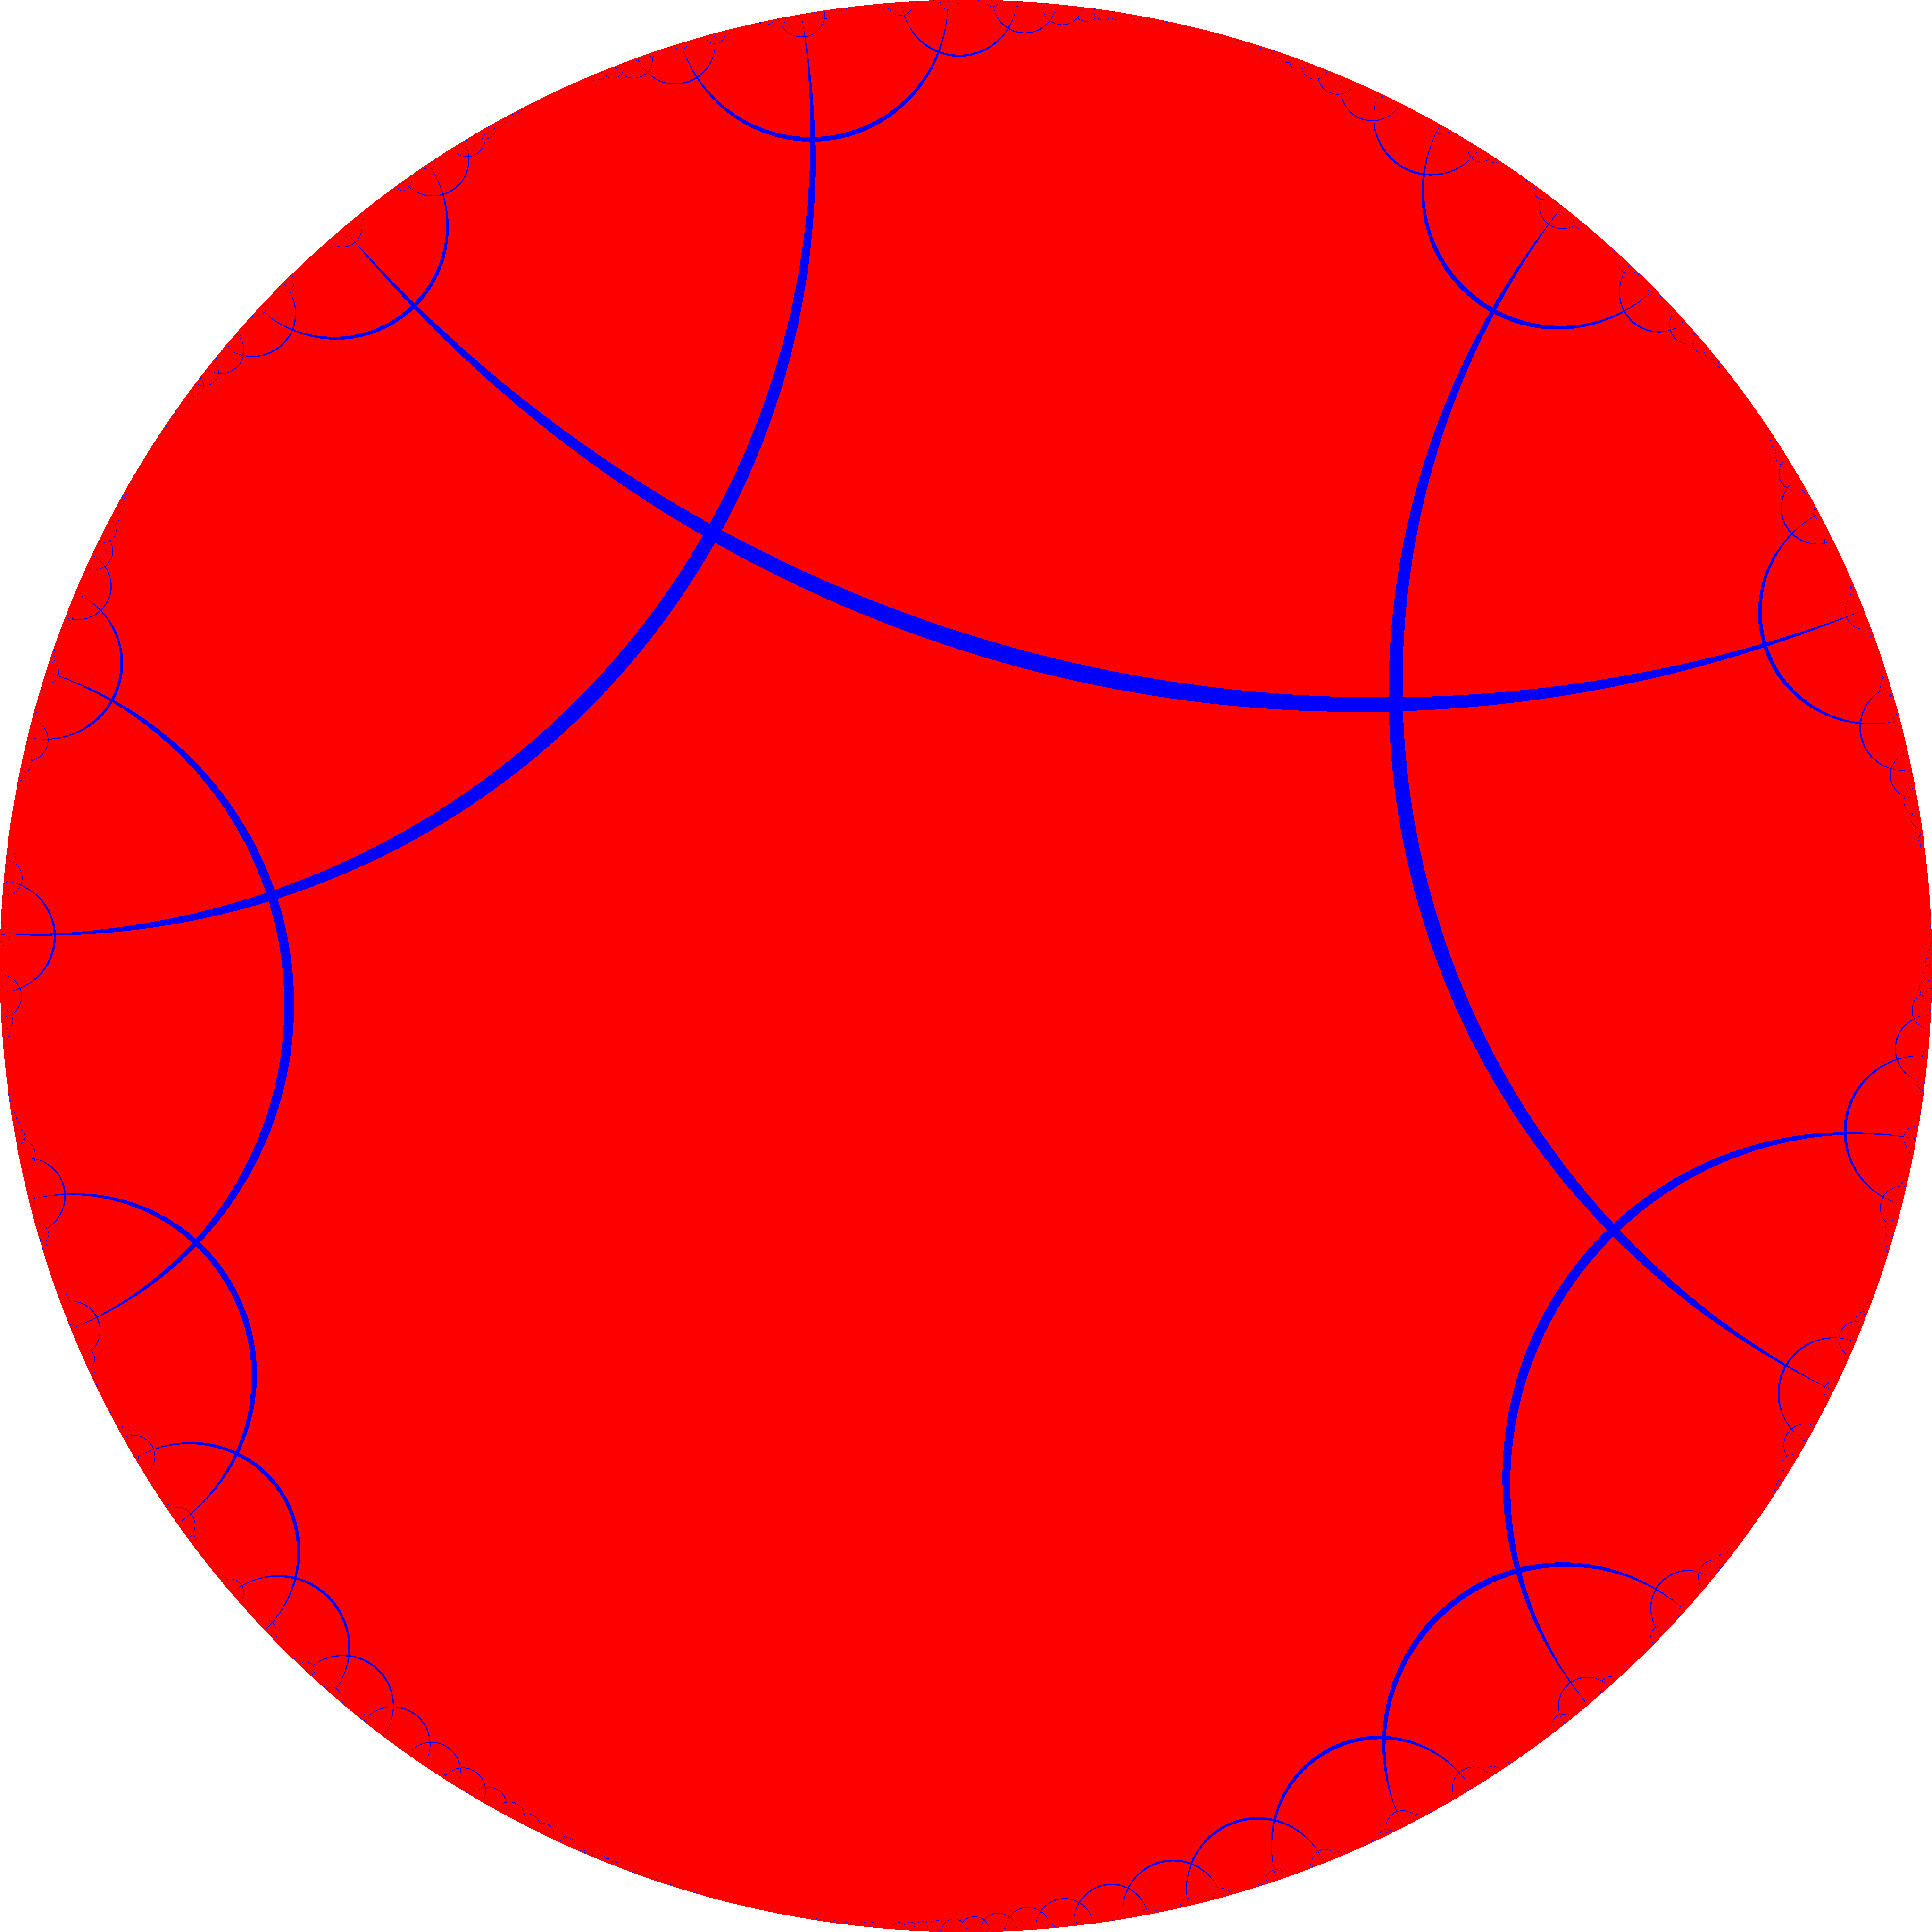
\includegraphics[width=6in]{images/t4096.png}};
    \draw (1.00, 2.60) node[inner sep=1pt] (p_z) {$+\frac{1}{2}$};
    \draw (-3.4, +3.9) node {$-\frac{1}{2}$};
    \draw (+5.2, +1.8) node {$+\frac{3}{2}$};

    \draw (-0.9, +6.2) node {$+0$};
    \draw (-1.9, +2.9) node {$+0$};
    \draw (-5.0, +0.3) node {$+0$};
    \draw (-7.0, +0.0) node {$+0$};

    \draw (+3.7, +4.9) node {$+2$};
    \draw (+3.1, +1.7) node {$+1$};
    \draw (+5.2, -2.5) node {$+\frac{1}{2}$};

    \draw (+0.00, +0.00) node {$+\frac{1}{4}$};

    % geodesic 0 %
    \draw [black, dotted, line width=1mm]
          (-1.89, -7.39) node[inner sep=1pt] (p_pinf) {}
       -- (+1.89, +7.39) node[inner sep=1pt] (p_ninf) {};

    % geodesic 1 %
    \draw [black, dotted, line width=1mm]
          (-3.29, 6.84) arc (205.0:58.7:-2.20);

    % line 0 %
    \draw [green, dotted, thick]
          (-3.29, 6.84) arc (240:271.7:18.00);

    % geodesic 1 %
    \draw [black, dotted, line width=1mm]
          (7.58, 0.55) arc (265.0:135.7:2.25);

    % line 0 %
    \draw [green, dotted, thick]
          (-3.29, 6.84) arc (240:271.7:18.00);

   % line 1 %
    \draw [green, dotted, thick]
          (-6.43, 4.05) arc (240:271.7:26.50);

   % line 2 %
    \draw [green, dotted, thick]
          (6.30, -4.30) arc (240:272.7:-25.50);

   % line 3 %
    \draw [green, dotted, thick]
          (4.38, -6.15) arc (240:273.0:-20.30);
\end{tikzpicture}
\caption{嵌入$1 + 2^{-n}$}
\end{figure}

\newpage

\section{共形嵌入的证明}

上面的构造过程蕴含了共形嵌入的证明思路,在此我们给出严格的证明。

\newpage

\section{环与扩域的想法}

\subsection{基础元素}

$\begin{array}{|c|c|}\hline 1&\space\\\hline n&0\\\hline\end{array} \mapsto n$ 代表整数,整个树都是整数值 $n$

$\begin{array}{|c|c|}\hline0&\space\\\hline 1&0\\\hline\end{array} \mapsto h$ 代表全体横向测地线(加线)的过滤器

$\begin{array}{|c|c|}\hline0&\space\\\hline 0&1\\\hline\end{array} \mapsto i$ 代表全体横向测地线(加线)上的自然增加

$\begin{array}{|c|c|}\hline2&\space\\\hline 1&0\\\hline\end{array} \mapsto j$ 代表全体纵向测地线(乘线)上的自然增加

$\begin{array}{|c|c|}\hline2&\space\\\hline 0&1\\\hline\end{array} \mapsto q$

$p$ 是将 $q$ 的加乘位置互易得到

\subsubsection{问题}

$o_p$ 独点的过滤器存在吗?其中 $p$ 是从原点到达该点路径的二进制编码

$g_p$ 单独一条测地线的过滤器存在吗?其中 $p$ 是从原点到达测地线的路径的二进制编码

$n$ 自己可以构成域,$n$ 与 $q$ 的组合能生成域吗?$n$ 与 $p$、 $q$ 的组合能生成域吗?

生成域的目标是包含 surreal number。

\newpage

\section{几个研究的方向}

任何一个程序的计算过程体现为一个流动,而且非常可能是一个保体积的流动。

1、初等数学:用函数式的观点,理解计算流动过程,重新考察初等几何、线性代数、微积分和微分方程等。比如圆是什么?线性是非常值得考察的。

2、计算理论:Chaitin 常数 $\Omega$ 的几何位置在哪里?

3、复变函数:庞加莱圆盘可以看成复平面上的单位圆盘,黎曼共形映射定理,直觉上,应该会有一个非常简洁的证明。

4、优化与变分:重新考察优化与变分,前传、后传。重要的是,大自然本身是优化过程,拉氏量的最小化。

5、学习理论:学习过程体现为一个反复迭代的程序,是测地线上的流动,重新考察学习的概念。

6、几何学:$H_2$上的保体积流和测地线流的研究会带来什么?

\end{document}
